\documentclass[twocolumn]{article}
\usepackage[margin=0.65in]{geometry}
\usepackage[T1]{fontenc}
\usepackage[utf8]{inputenc}
\usepackage[UKenglish]{babel}
\usepackage{graphicx}
\usepackage[tight]{subfigure}
\usepackage{hyperref}
\usepackage{amsmath}
\usepackage{amssymb}
\usepackage{float}
\usepackage[skip=5pt]{caption}
\usepackage{authblk}
\usepackage{comment}

\title{Human body shapes anomaly detection and classification using persistent homology}
\author[1,2]{Steve de Rose}
\author[1]{Philippe Meyer}
\author[1]{Frédéric Bertrand}
\affil[1]{Computer Science and Digital Society Laboratory (LIST3N), Université de Technologie de Troyes, Troyes, France}
\affil[2]{Institut de Recherche Mathématique Avancée
 (IRMA), CNRS UMR 7501, Université de Strasbourg, Strasbourg, France}
\date{}

\begin{document}

\maketitle

\begin{abstract}
In this paper, we use topological data analysis to study human body shapes. Persistence theory applied on anthropometric point clouds together with clustering algorithms show that relevant informations about shapes are extracted by persistent homology. In the first place anomalies of scans are detected using complete-linkage hierarchical clusterings. Then, a discrimination index shows which type of hierarchical clustering separate gender accurately. Finally, Ward-linkage hierarchical clusterings with Davies-Bouldin, Dunn and Silhouette indices are used to define 8 groups of men morphotypes and 7 groups of women morphotypes.
\end{abstract}

\section{Introduction}

The separation of human bodies into groups of morphologies is a common issue for garment industries. Rather than targeting a single standard body shape, the discrimination of morphologies helps to improve sizing systems and can reduce production costs to apparel manufacturing.

Among the classifications already established, there is one from \cite{SKO04} particularly used by industries where the authors obtained 9 types of female body shapes such as triangle, inverted triangle, hourglass, oval, etc. This is the first work where mathematical criteria, together with the help of experts, have been used to define these groups.
\vspace{0.2cm}

In terms of data science, we can approach this problem by clustering algorithms. To this end different types of data can be extracted from a body such as measurements or anthropometric point clouds.

Body measurements can be directly represented in an euclidean space to use methods from data analysis. In \cite{SA11}, principal component and K-means cluster analyses are performed on measurements and key body locations and 3 women lower body shape groups are obtained.

On the other hand, to cluster human bodies from 3D-dimensional representations we need a way to extract information from anthropometric point clouds and to compare them.

For example, in \cite{NK09} the authors use control points and correlation strength principal component analysis of trunks. Reinterpreting these components by averaged shape figures and combining factor loading maps, 5 women trunk shape groups are defined by a Ward-linkage hierarchical clustering.

Different methods from data science have been used to classify human body shapes, see for example \cite{C12}, \cite{HTB17}, \cite{NZHBNIS18} and \cite{PPA19}.
\vspace{0.2cm}

Topological data analysis \cite{CM21}, \cite{M17} is a powerful tool to study and understand the shape of data and thus it naturally applies in this context. In particular, persistent homology \cite{ELZ02}, \cite{ZC05} can be used to extract relevant topological informations from data and point clouds. These extracted features are encoded by diagrams and have stability properties relatively to specific distances \cite{CSEHH05}, \cite{CCSGGO09}.

Several applications of this theory have been established in different contexts such as time-series data analysis \cite{UKK19}, object recognition \cite{LOC14}, complex network analysis \cite{HMR09} and molecular biology data exploration \cite{YSHBSLGPC09}.
\vspace{0.2cm}

In this work, after explanations in Section \ref{sec:methodology} about persistence diagrams, Wasserstein distance and associated silhouettes, we apply tools from persistence and clustering theories on the human point clouds of the CAESAR database \cite{YYZDDY14}. Approaches by homological degree, using graph theory among other things, allow us to interpret persistent homologies and identify them to body areas and limbs. To define morphotypes independently of individuals height we normalize the point clouds using three-dimensional homotheties.

In Section \ref{sec:anomaly}, we show that anomalies of scans are naturally isolated clusters when performing complete-linkage hierarchical clustering on the persistence diagrams of the point clouds using the Wasserstein distance.

Then a gender discrimination index is defined in Section \ref{sec:GDI} to study which hierarchical clustering linkage is interesting to separate accurately males and females. We compare the performance of these clustering algorithms on persistence diagrams, on silhouettes, and also if point clouds are restricted to trunks or not.

Finally, in Section \ref{sec:classification}, Ward-linkage hierarchical clusterings on the silhouettes of the persistence diagrams of the point clouds, together with a mix of different clustering criteria such as Davies-Bouldin, Dunn and Silhouette indices are used to obtain 8 men morphotypes and 7 women morphotypes. Then we study properties of these clusters and their medoids are computed and considered as representatives of the groups.

\section{Methodology} \label{sec:methodology}

\subsection{Dataset}

The CAESAR (Civilian American and European Surface Anthropometry Resource) 3D Anthropometric Database is composed of 3D body scans of thousands of men and women aged from 18 to 65 and originated from various NATO countries: the United States of America, Canada, the Netherlands and Italy.

In this paper we are using the dataset of \cite{YYZDDY14} which is derived from the CAESAR dataset and is composed of 1517 male and 1531 female meshes, registered as OBJ files. Each mesh has 12500 vertices (Figure \ref{fig:mesh+cloud_points}.(a)) and 25000 faces (Figure \ref{fig:mesh+cloud_points}.(b)) and we will just extract and consider the underlying point clouds of all the meshes. In Figures the meshes and point clouds are presented headless for confidentiality. The individuals are numbered discontinuously from {\tt Spring0001} to {\tt Spring4800} and for convenience we refer to {\tt SpringXXXX} by {\tt SXXXX}.

\begin{figure}[H]
    \centering
    \subfigure[The vertices]{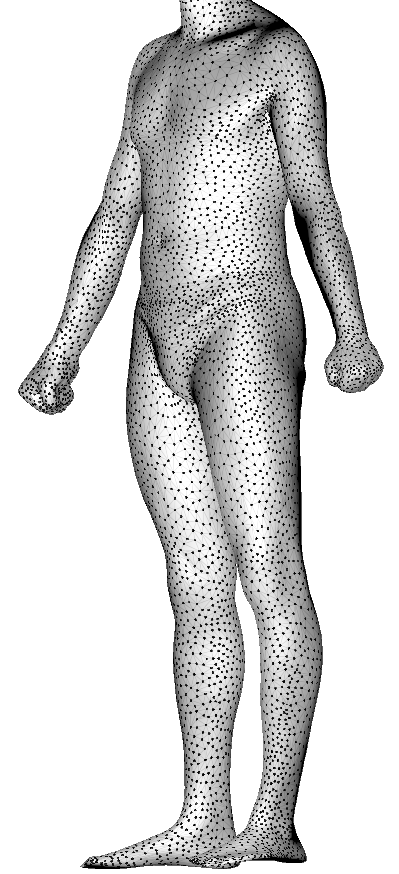
\includegraphics[height=.25\textheight]{img/cloudpoints_S0013.png}}\qquad
    \subfigure[The faces]{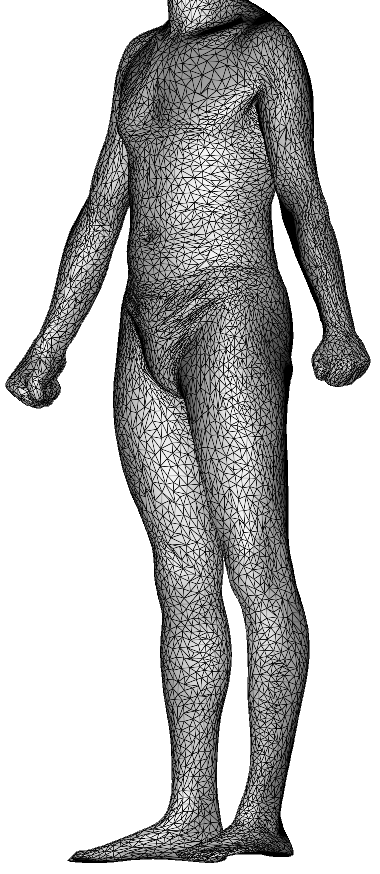
\includegraphics[height=.25\textheight]{img/mesh_S0013.png}}
    \caption{The mesh of the individual {\tt S0013}.}
    \label{fig:mesh+cloud_points}
\end{figure}

\subsection{Persistence diagrams, landscapes, silhouettes and distances}

Persistent homology is a tool used to efficiently compute and encode the multidimensional homological features of topological spaces associated to a dataset.

To compute these homological invariants, we have to build topological structures on the data such as filtered simplicial complexes. These invariants are then represented by a persistence barcode or a persistence diagram. For example in Figure \ref{fig:PD+PB} are the persistence barcode and diagram of the individual {\tt S0013} represented in Figure \ref{fig:mesh+cloud_points}.

\begin{figure}[H]
    \centering
    \subfigure[Persistence diagram]{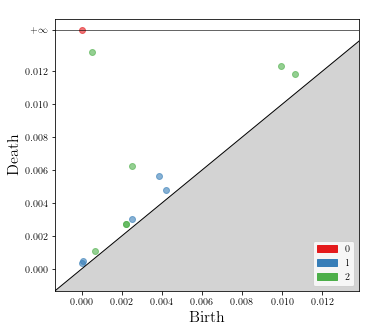
\includegraphics[height=.165\textheight]{img/PD_S0013_d.png}}
    \subfigure[Persistence barcode]{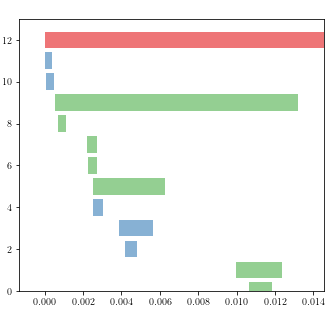
\includegraphics[height=.165\textheight]{img/PD_S0013_b.png}}
    \caption{The persistence diagram and barcode of {\tt S0013}.}
    \label{fig:PD+PB}
\end{figure}

The persistence in dimension $0$ is related to the number of connected components, in dimension $1$ it describes non-homotopic loops and in dimension $2$ it characterizes $2$-dimensional voids.

The persistence barcode represents each homology class of the 1D-parameterized family of topological spaces obtained from the point cloud with a bar defined by its birth time, when the topological feature appears, and a death time, when the topological feature disappears. From this we represent each bar by a point in $\mathbb{R}^2$ where its abscissa is the birth time, its ordinate is the death time. The set of points obtained in this way is referred as the persistence diagram.

It is possible to compare persistence diagrams using the Wasserstein distance. Let $D$ and $D'$ be persistence diagrams and let $\Phi$ be the set of perfect matchings between them, completing with the diagonal if necessary. The $(p,q)$-Wasserstein distance between $D$ and $D'$ is defined by
\begin{equation*}
    W_{p,q}(D,D')=\underset{\phi \in \Phi}{inf}(\sum\limits_{x \in D} ||x-\phi(x)||^p_q)^{1/p}.
\end{equation*}

We will use exclusively the $(2,2)$-Wasserstein distance. For precise definitions and details, see \cite{CM21} and \cite{M17}.
\vspace{0.2cm}

Persistence landscapes are an encoding of persistence diagrams by series of piecewise continuous linear functions \cite{CFLRW14}, \cite{B15}, see Figure \ref{fig:persistence_landscape}. This allows us to perform statistics on them, the absence of which was a disadvantage of persistence diagrams. In particular, it is possible to calculate unique averages of landscapes. While a persistence landscape has a corresponding persistence diagram, an average of persistence landscapes does not.

\begin{figure}[H]
    \centering
    \subfigure{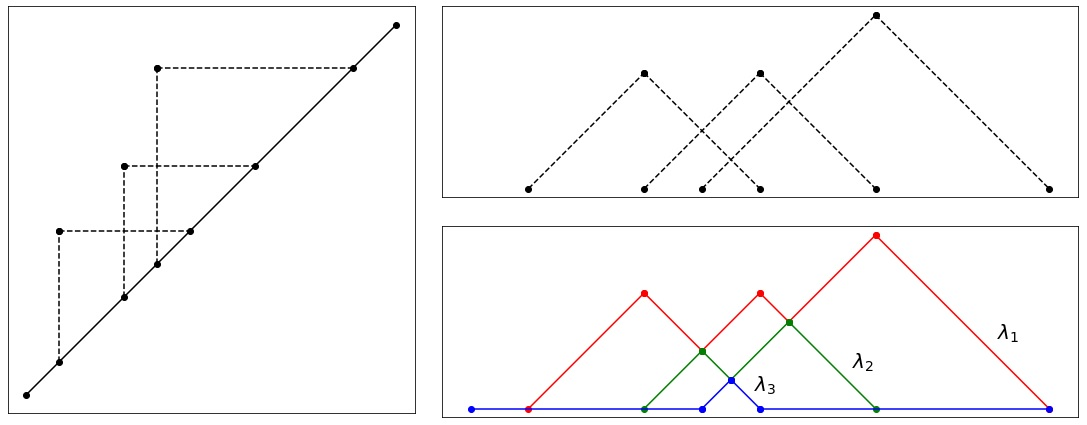
\includegraphics[width=.48\textwidth]{img/pl.png}}
    \caption{Visual explanation of persistence landscapes. The persistence diagram (left) is tilted, so that the diagonal becomes the new horizontal axis (top right). The $\lambda_i$ are the piecewise linear functions (bottom right).}
    \label{fig:persistence_landscape}
\end{figure}

A persistence silhouette is computed by taking a weighted average of the collection of 1D-piecewise-linear functions given by the persistence landscapes, and then by evenly sampling this average on a given range. Finally, the corresponding vector of samples is returned, see Figure \ref{fig:persistence_silhouette}.

For the implementation of clustering, we choose to make a vector consisting of 25 points of the silhouette of $H_0$ homologies, 250 points equidistant from the silhouette of $H_1$ homologies and 250 points equidistant from the silhouette of $H_2$ homologies, for each persistence diagram. The points are the values of the silhouette equally spaced.

\begin{figure}[H]
    \centering
    \subfigure{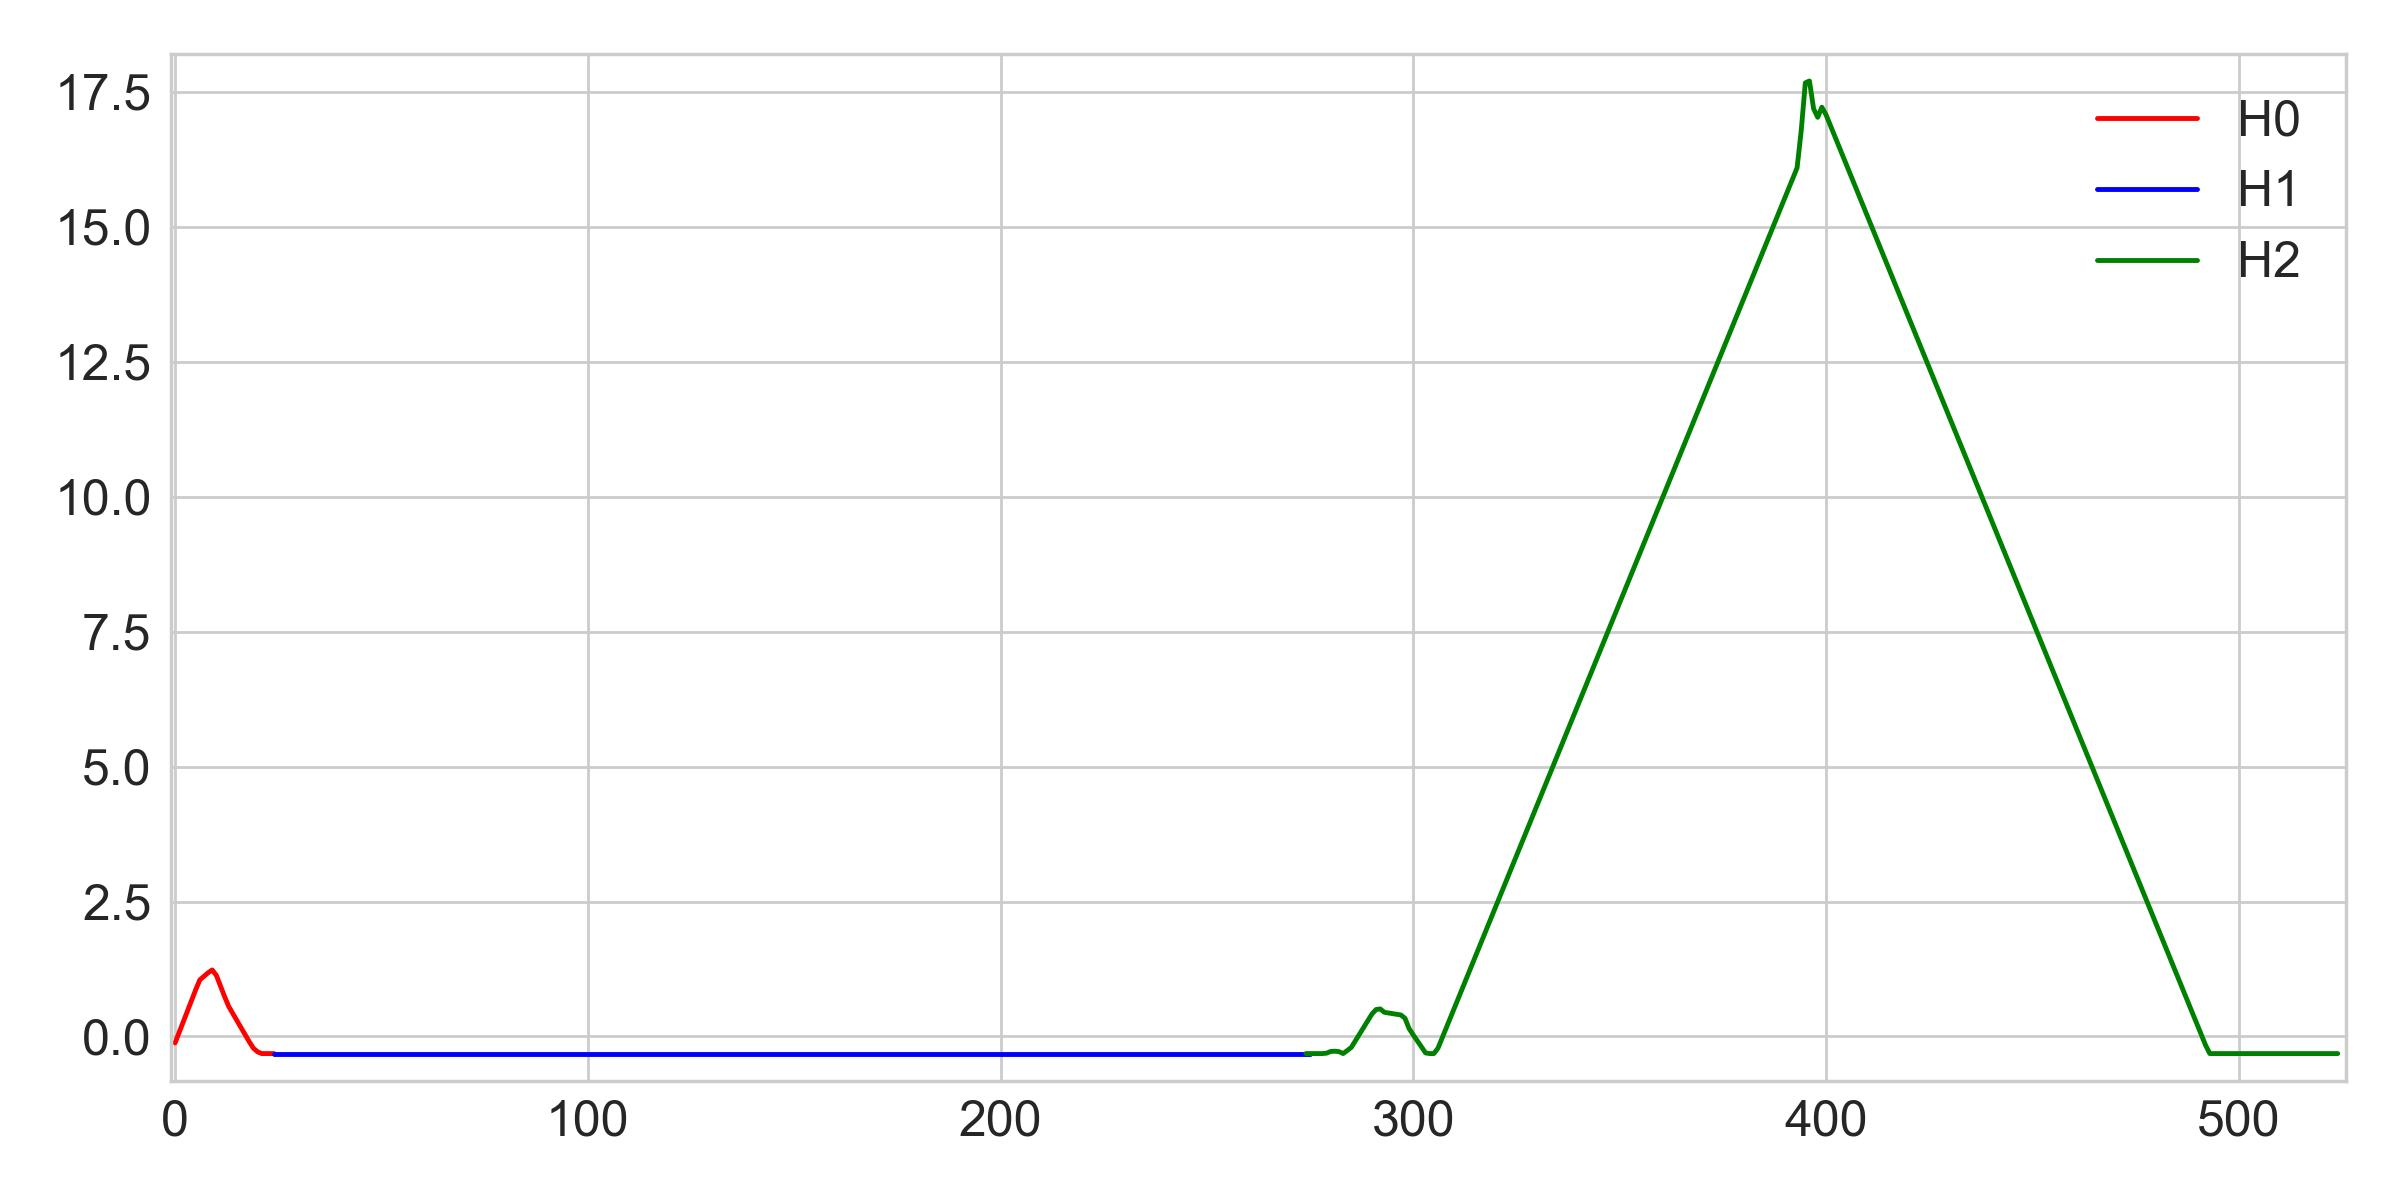
\includegraphics[width=.49\textwidth]{img/temp/pl2.png}}
    \caption{Representation of a vector obtained by persistence silhouette.}
    \label{fig:persistence_silhouette}
\end{figure}

\subsection{Interpretation of persistent homology}

Since displaying the homologies in their entirety is too costly, we thought of other approaches for each degree.

For each homology, we know the radii of the balls at its birth and death. A simplex tree represents abstract simplicial complexes of any dimension. All faces of the simplicial complex are explicitly stored in a trie whose nodes are in bijection with the faces of the complex. This data structure allows to efficiently implement a large range of basic operations on simplicial complexes. Using the simplex tree of a set of points, we know the values of the radii when pairs of points, triangles and tetrahedra are covered. The approach is slightly different depending on the dimension:

\begin{itemize}
\setlength\itemsep{-0.25em}
    \item Dimension 0: All $H_0$ homologies are born when the radius of the balls is zero. For each homology $H_0$, we choose to display the second point of the pair covered at the birth of the homology as its representative.
    \item Dimension 1: First, we make an undirected graph containing all the points of a set, where each time a pair of points is covered, as the radius of the balls increases, we connect these points by an edge with a weight equal to the radius of the balls. At the birth of a homology $H_1$, before adding the edge to our graph, we compute the shortest path connecting these two points which we display by closing it with the segment connecting these points. The lace displayed is a likely representative of this homology. At the death of this homology, we recover the information of the triangle covered by the balls and we add it to the display to give a general idea of the evolution of our homology.
    \item Dimension 2: For each homology $H_2$, we simply display the triangle covered at its birth and the tetrahedron covered at its death.
\end{itemize}

\begin{comment}
\begin{figure}[H]   
    \centering
    \subfigure[$H_1$ n°5]{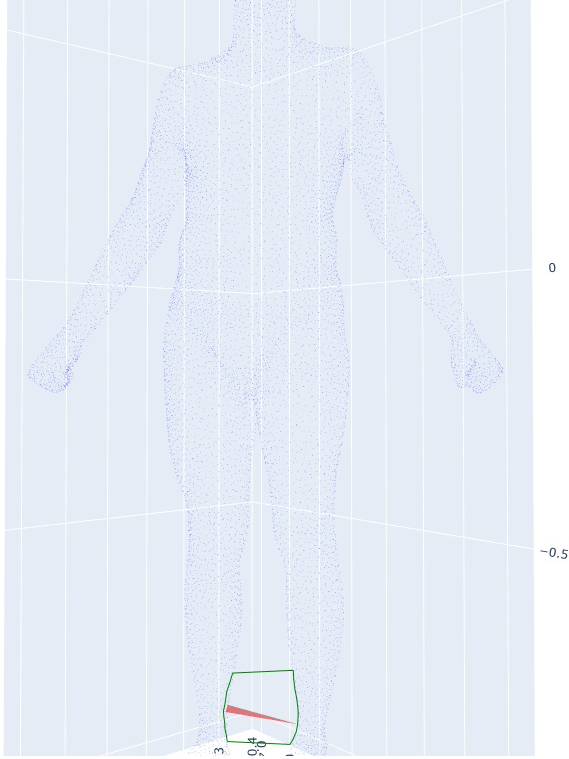
\includegraphics[height=.25\textheight]{img/temp/vishom1.png}}
    \subfigure[$H_2$ n°2]{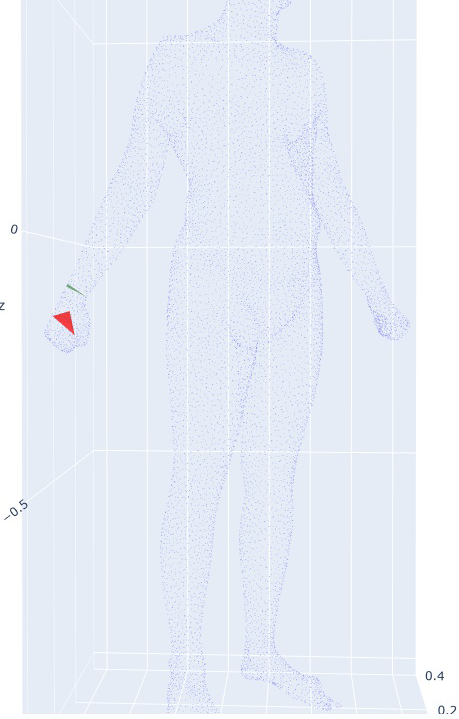
\includegraphics[height=.26\textheight]{img/temp/vishom2.png}}
    \caption{Examples of homology posters for an individual. The fifth homology $H_1$ on the left corresponds to the inter-ankle surface and the second homology $H_2$ on the right corresponds to the right hand volume.}
\end{figure}
\end{comment}

For example in the persistence diagram of the individual {\tt S0013} given in Figure \ref{fig:PD+PB}, there are 13 different homologies numbered in the persistence barcode from 0 to 12. With this approach we display each homology in Figure \ref{fig:S0013_hom_posters} and we can interpret them as follows:

\begin{itemize}
\setlength\itemsep{-0.25em}
    \item n°0: $H_2$ corresponding to the left part of the torso,
    \item n°1: $H_2$ corresponding to the right part of the torso,
    \item n°2: $H_1$ corresponding to a loop between legs at foot level,
    \item n°3: $H_1$ corresponding to a loop between legs from ankles to calves,
    \item n°4: $H_1$ corresponding to a loop between legs from knees to calves,
    \item n°5: $H_2$ corresponding to the head,
    \item n°6: $H_2$ corresponding to the right calf,
    \item n°7: $H_2$ corresponding to the left calf,
    \item n°8: $H_2$ corresponding to the right foot,
    \item n°9: $H_2$ corresponding to the whole body,
    \item n°10: $H_1$ corresponding to a loop around the right foot,
    \item n°11: $H_1$ corresponding to a loop around the left foot,
    \item n°12: $H_0$ of all the connected balls.
\end{itemize}

We remark that the arms and the left foot don't appear on the diagram. This is caused by the minimal persistence and the fact that the arms are too thin and that the scan of the left foot is more flat and deformed compared to the right one. The homology n°9 is particularly distinguished and we call it the principal $H_2$-homology. It corresponds to the aggregation of the parts and limbs of the body, thus forming the inner cavity of the body point cloud.

\begin{figure}[H]
    \centering
\subfigure[n°0]{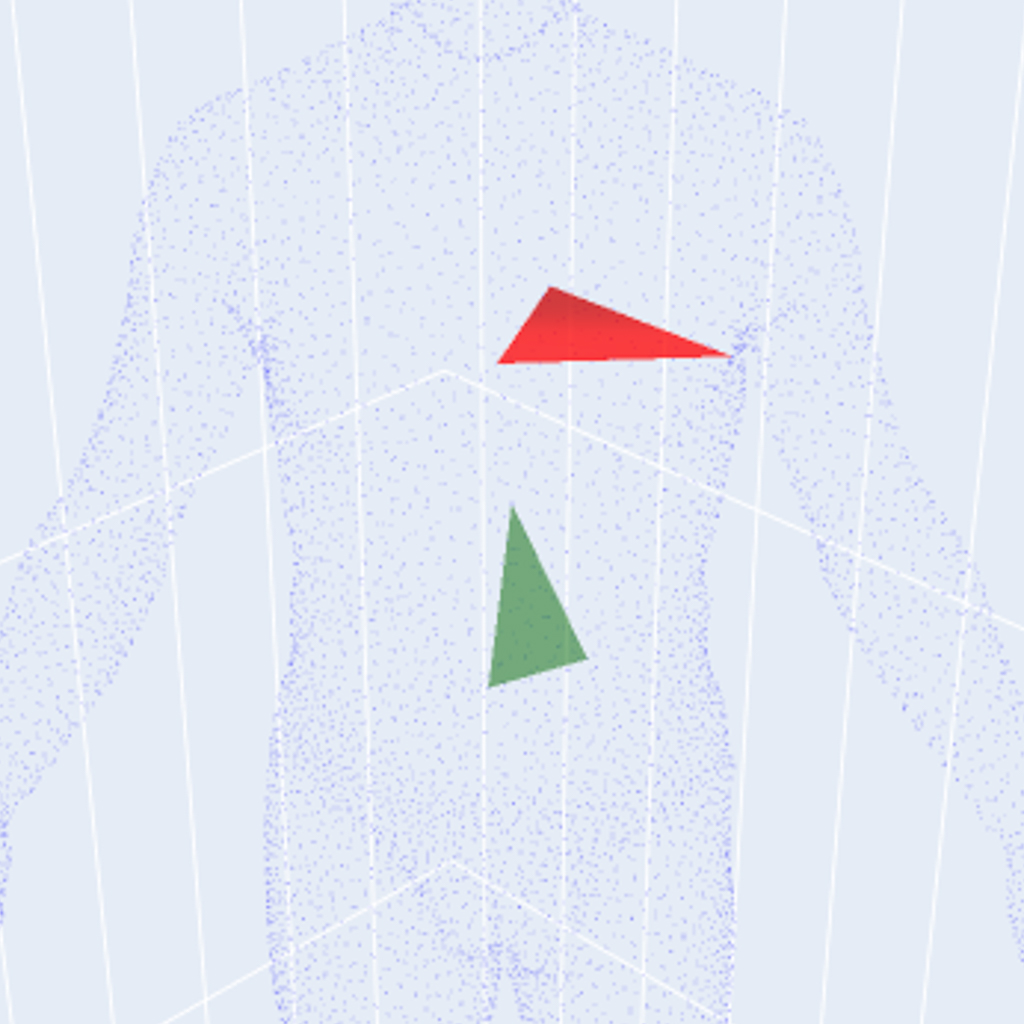
\includegraphics[height=.11\textheight]{img/interpretation/H2-6.jpg}}
\subfigure[n°1]{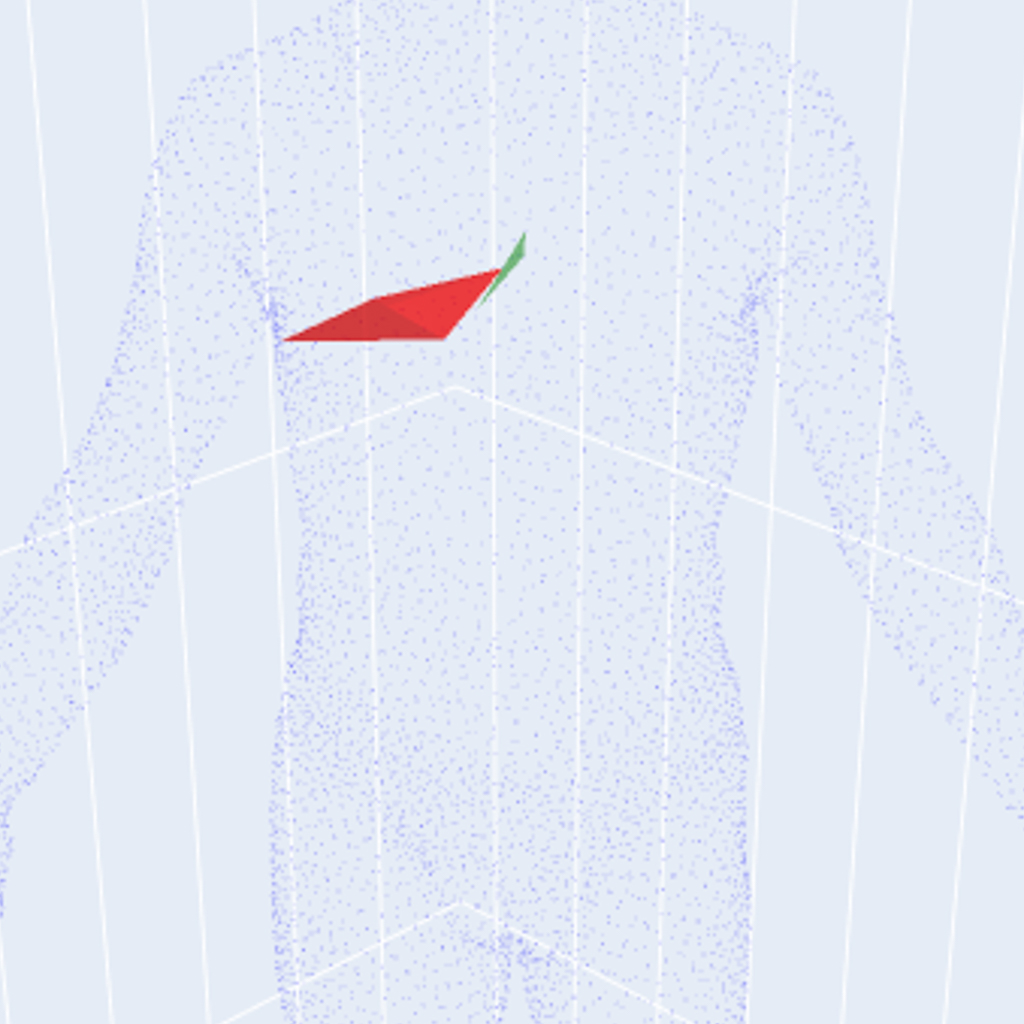
\includegraphics[height=.11\textheight]{img/interpretation/H2-7.jpg}}
\subfigure[n°2]{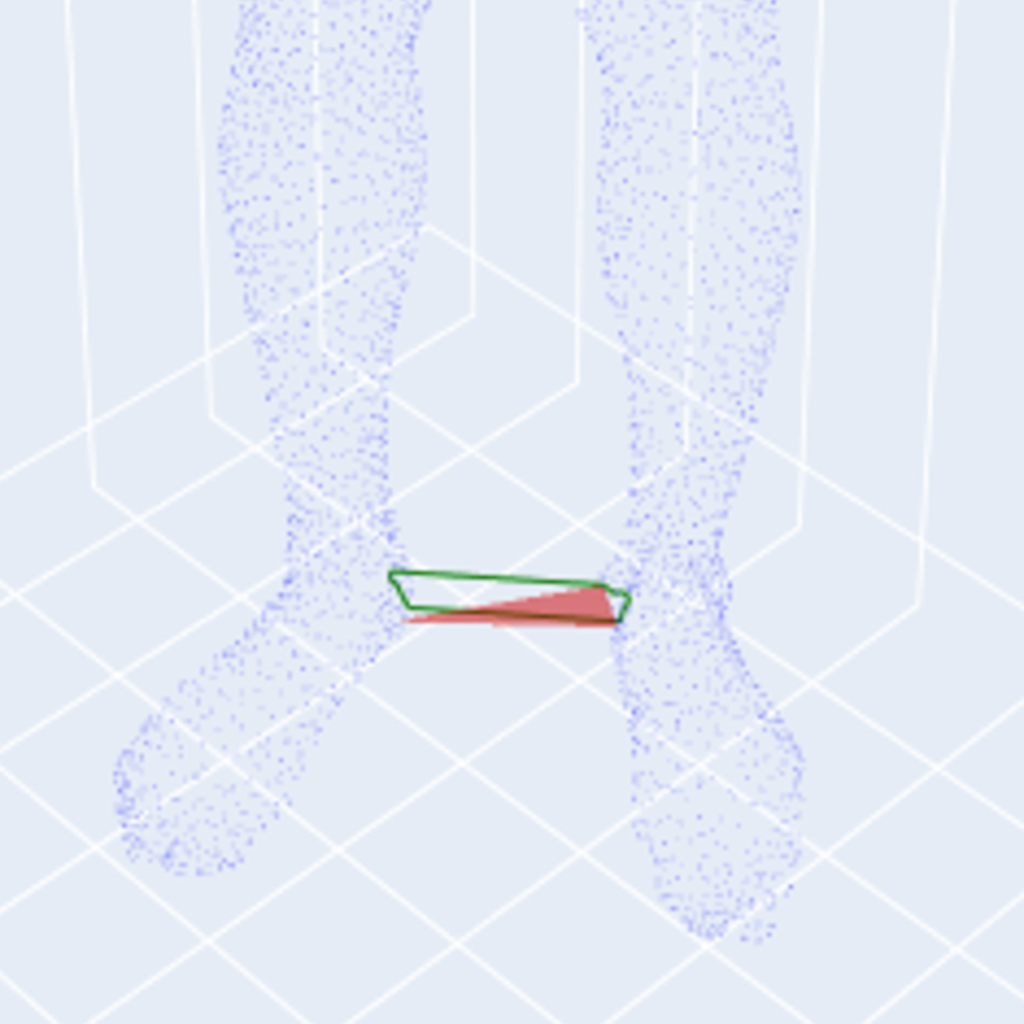
\includegraphics[height=.11\textheight]{img/interpretation/H1-5.jpg}}
\subfigure[n°3]{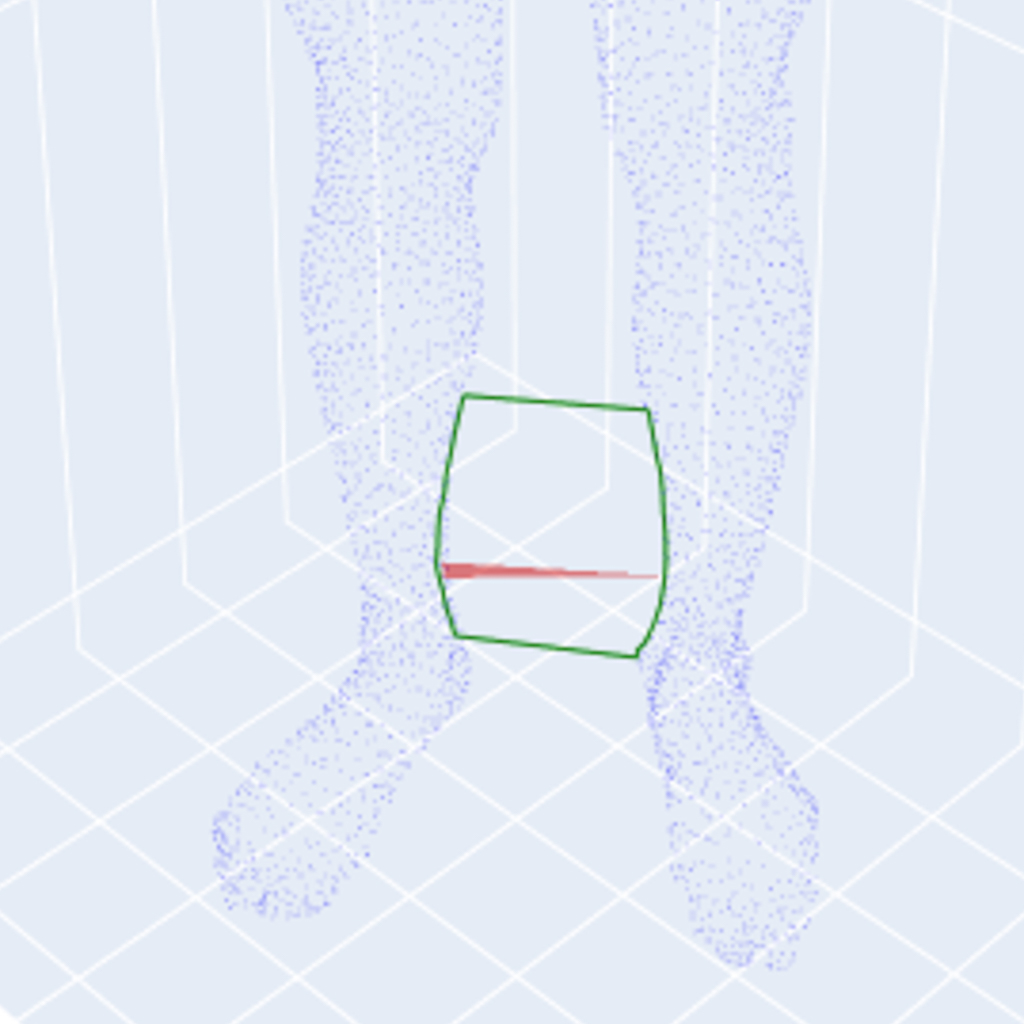
\includegraphics[height=.11\textheight]{img/interpretation/H1-4.jpg}}
\subfigure[n°4]{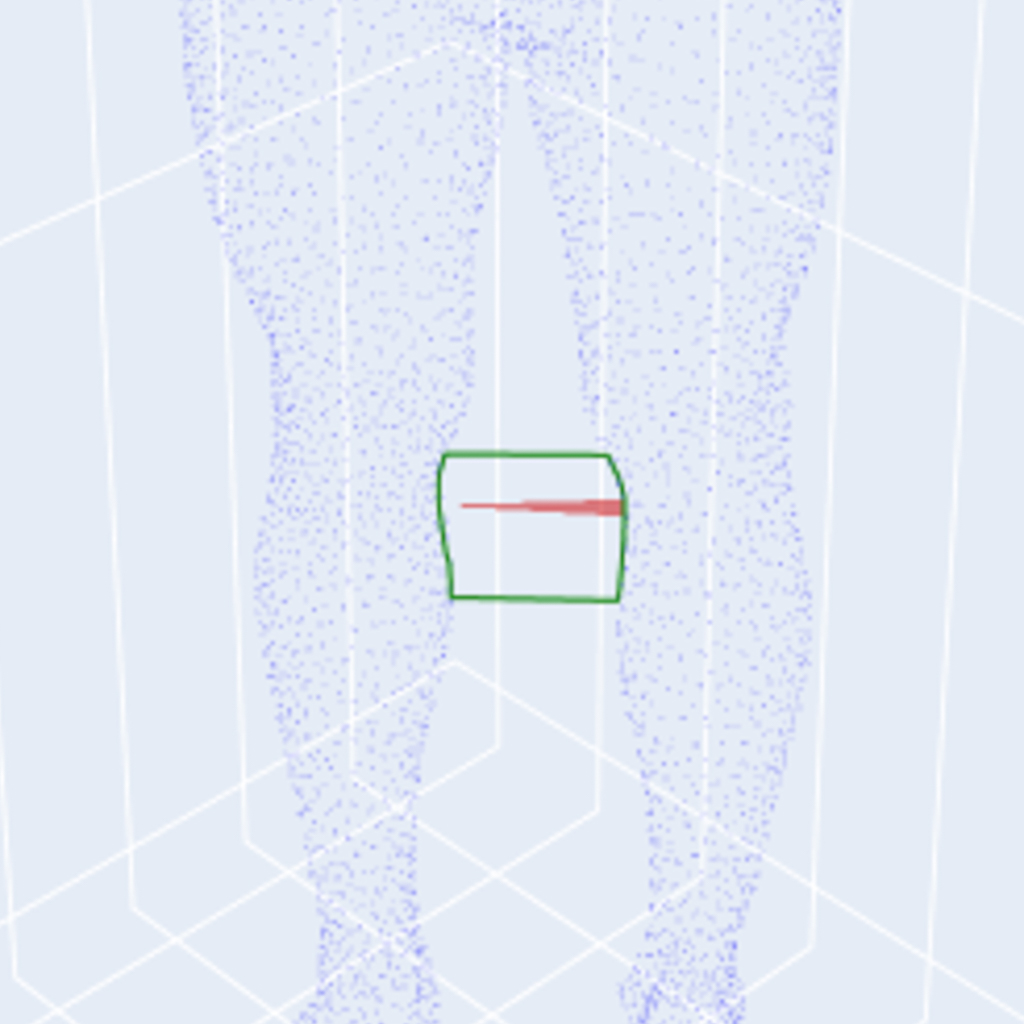
\includegraphics[height=.11\textheight]{img/interpretation/H1-3.jpg}}
\subfigure[n°5]{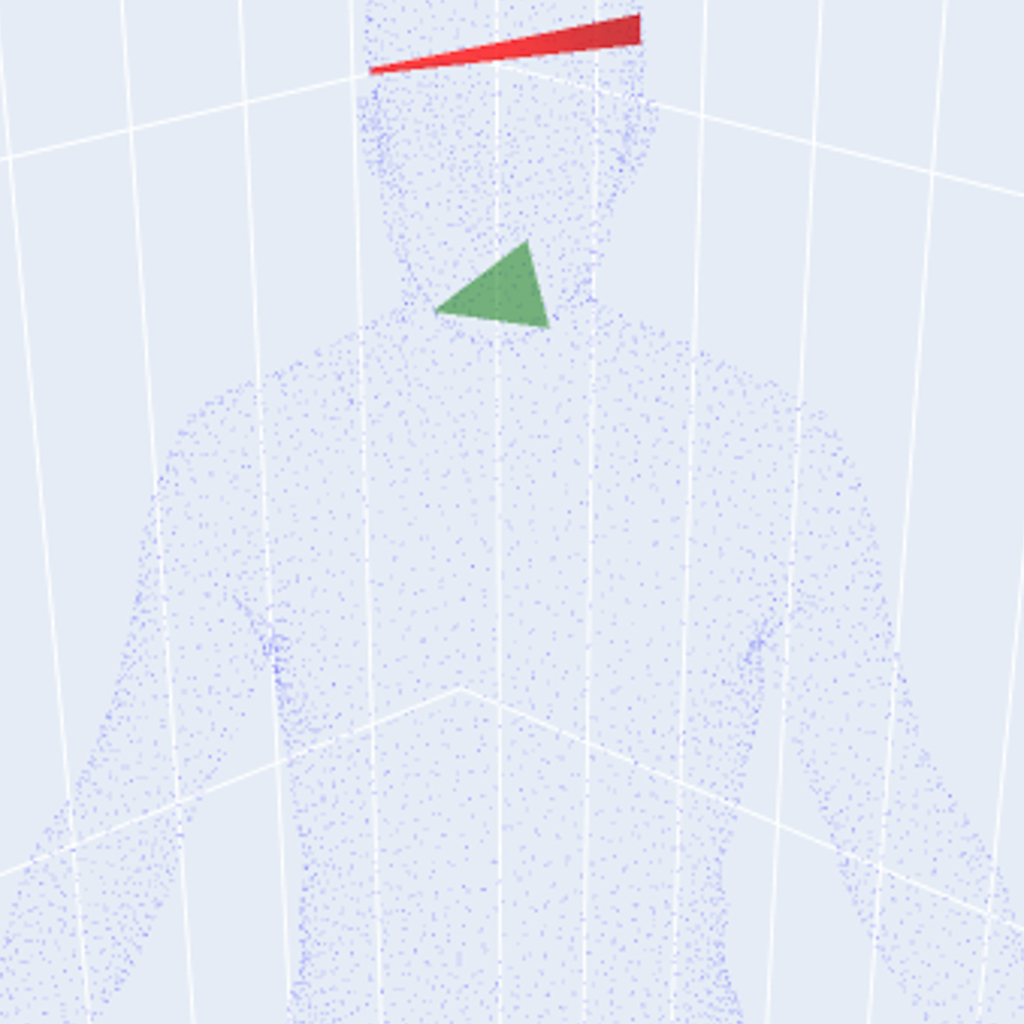
\includegraphics[height=.11\textheight]{img/interpretation/H2-5.jpg}}
\subfigure[n°6]{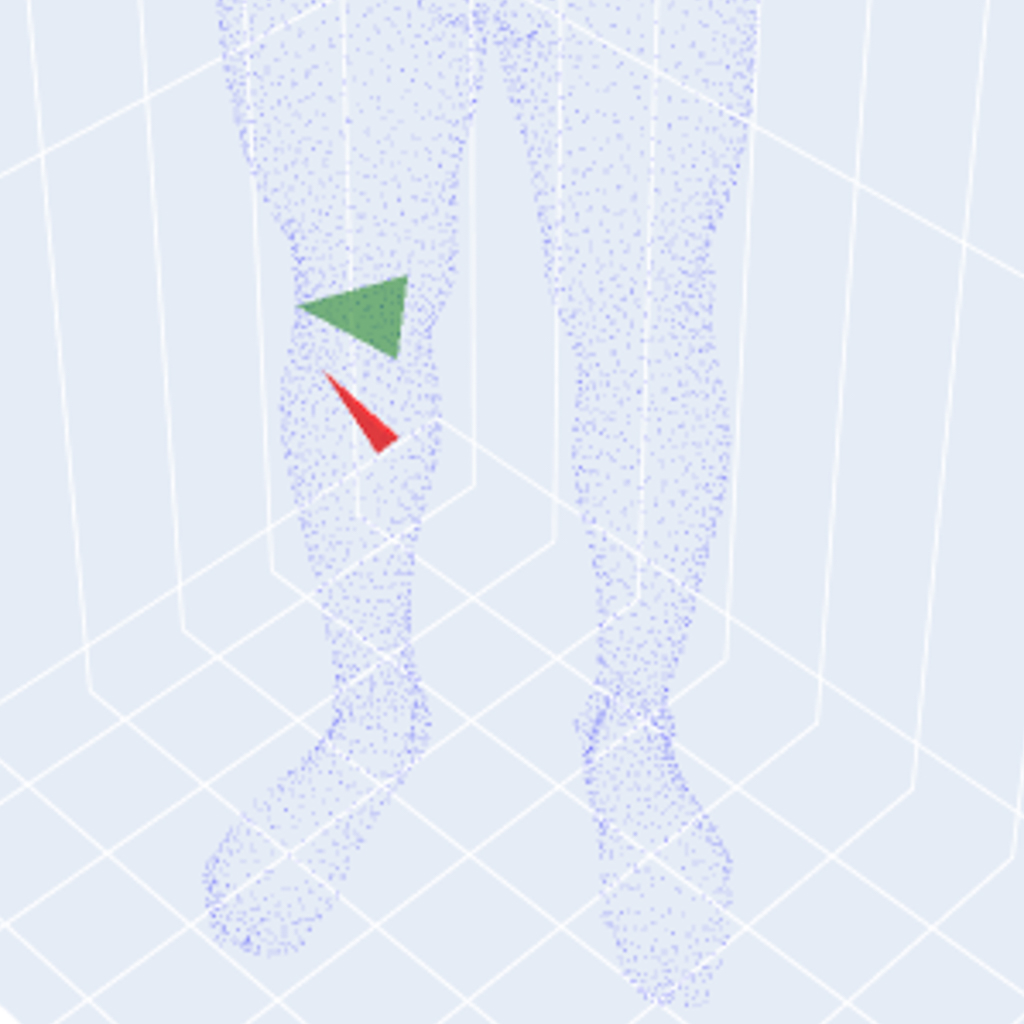
\includegraphics[height=.11\textheight]{img/interpretation/H2-4.jpg}}
\subfigure[n°7]{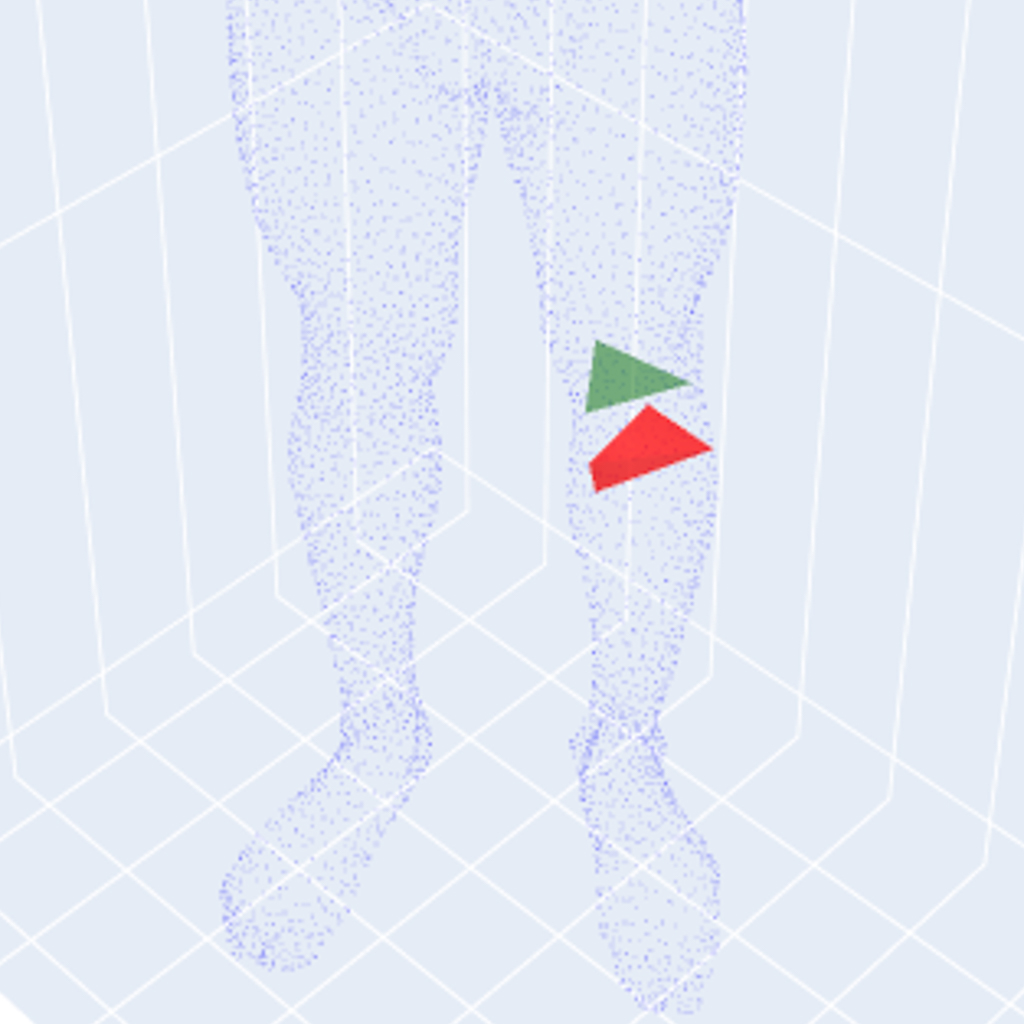
\includegraphics[height=.11\textheight]{img/interpretation/H2-3.jpg}}
\subfigure[n°8]{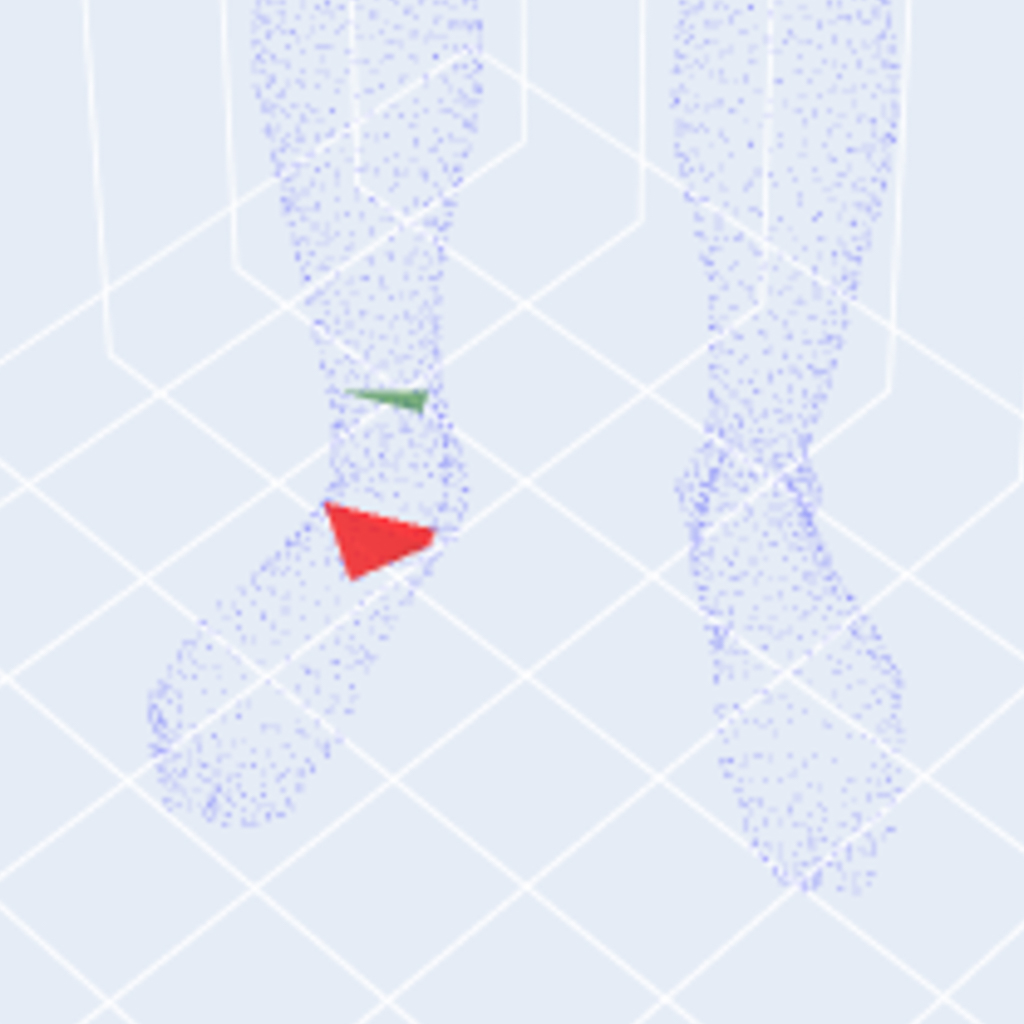
\includegraphics[height=.11\textheight]{img/interpretation/H2-2.jpg}}
\subfigure[n°9]{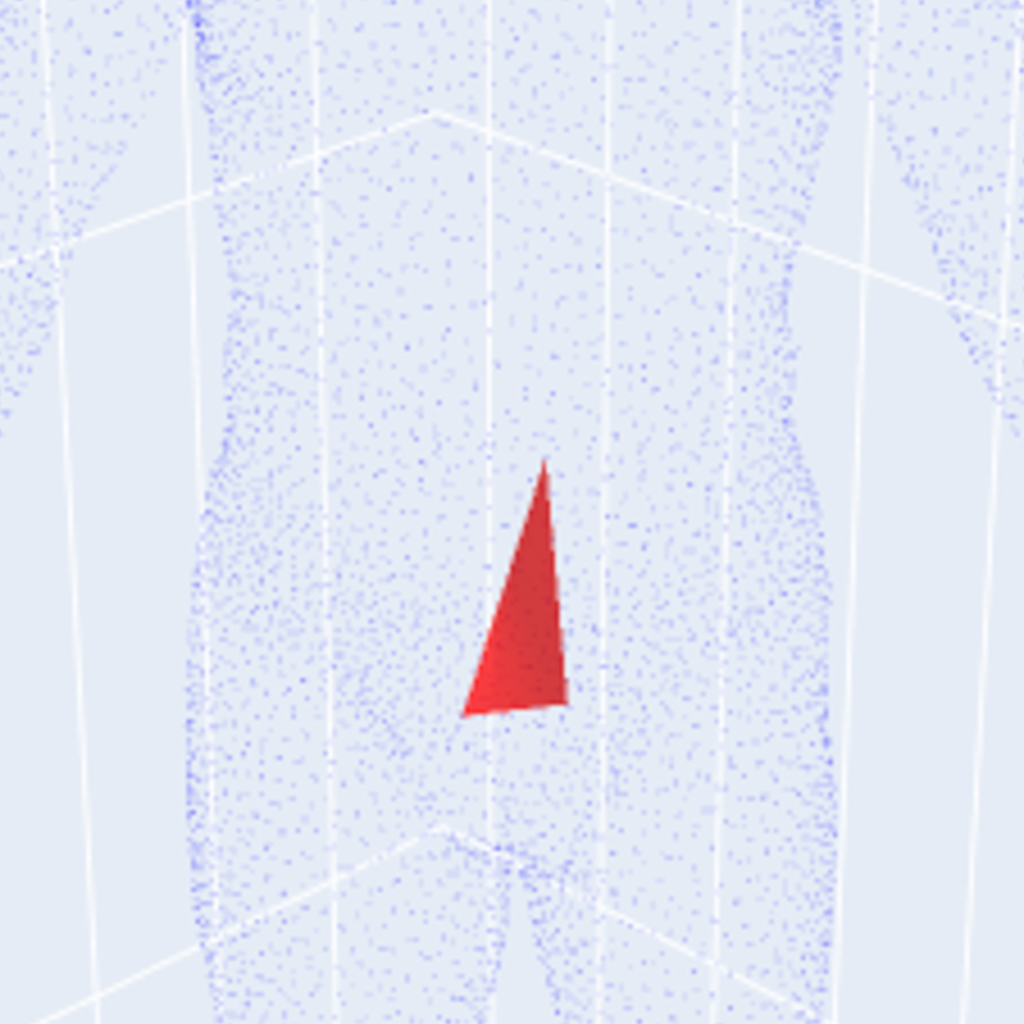
\includegraphics[height=.11\textheight]{img/interpretation/H2-1.jpg}}
\subfigure[n°10]{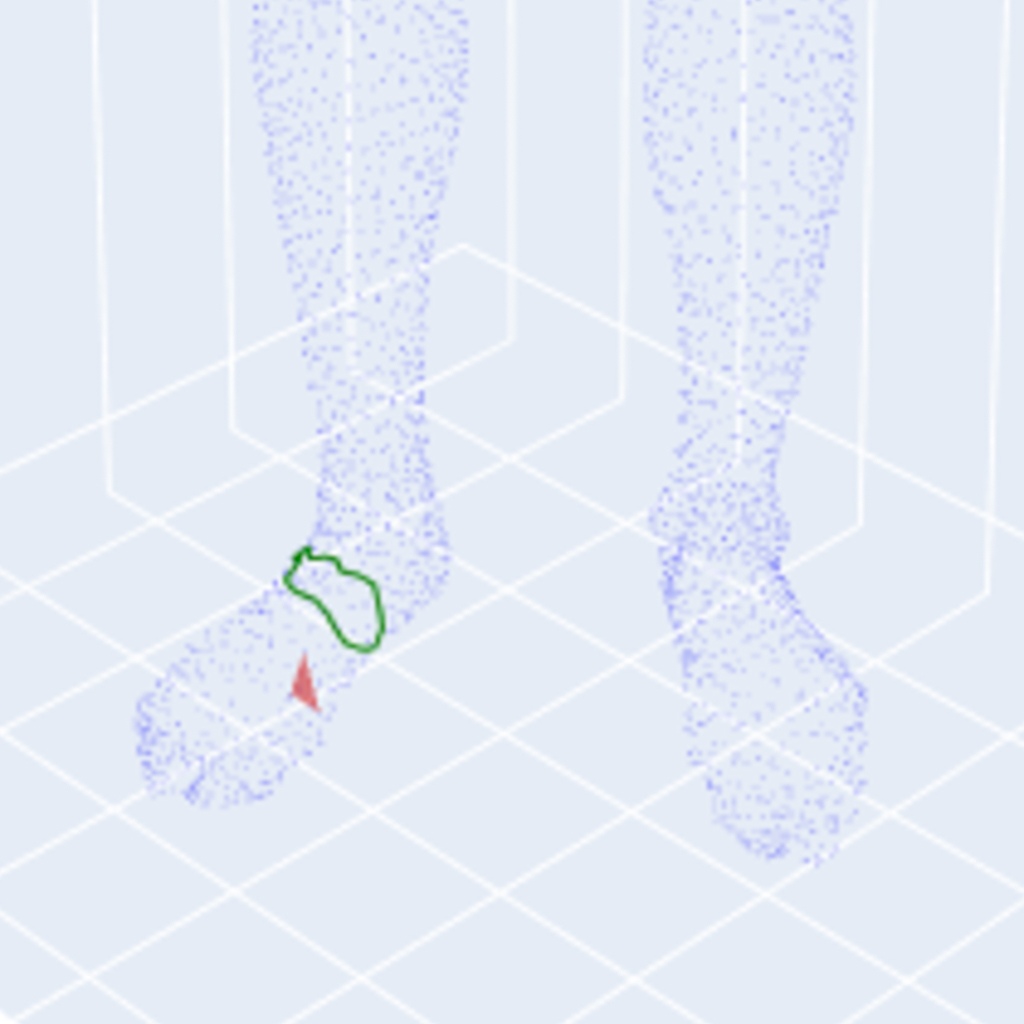
\includegraphics[height=.11\textheight]{img/interpretation/H1-2.jpg}}
\subfigure[n°11]{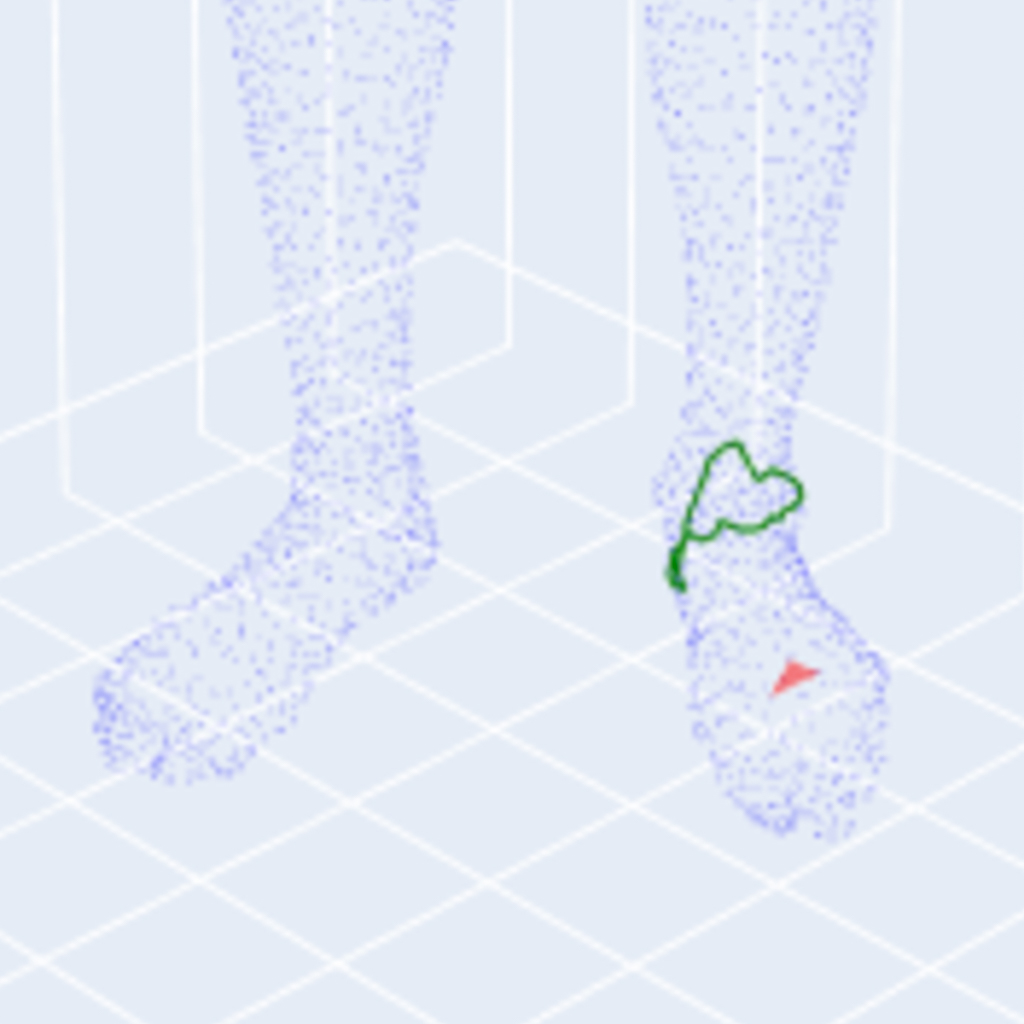
\includegraphics[height=.11\textheight]{img/interpretation/H1-1.jpg}}
    \caption{All non $H_0$ homologies of the persistence diagram of {\tt S0013}.}
    \label{fig:S0013_hom_posters}
\end{figure}

\subsection{Normalization of point clouds by homothety} \label{sec:normalisation}

We want morphotypes to be independent of the size of the individuals in order to propose a sizing system associated to each morphotype. For this purpose we apply a homothety on each point cloud so that each individual is the same height. This affects the distances between them and individuals with similar morphology but different height become closer (Figure \ref{fig:normalisation}). 

\begin{figure}[H]
    \centering
    \subfigure[\tt S0105]{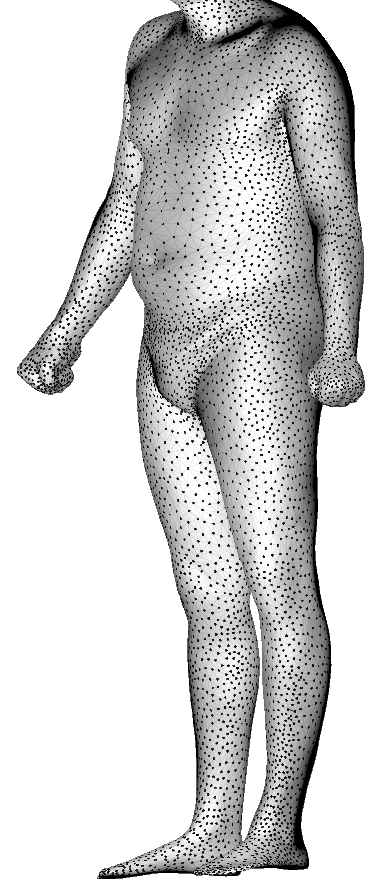
\includegraphics[height=.24192\textheight]{img/normalisation/SPRING0105.png}}\qquad
    \subfigure[\tt S0071]{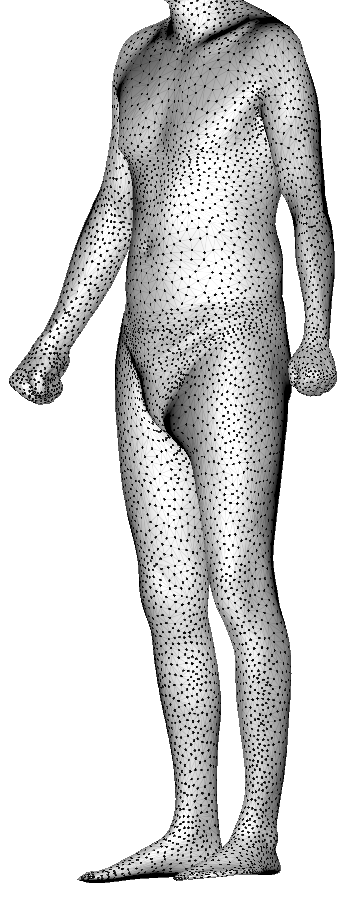
\includegraphics[height=.24704\textheight]{img/normalisation/SPRING0071.png}}\qquad
    \subfigure[\tt S0207]{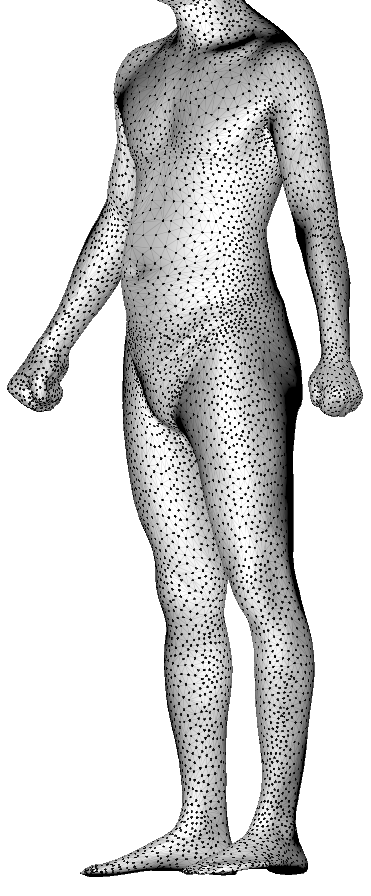
\includegraphics[height=.2112\textheight]{img/normalisation/SPRING0207.png}}
    \caption{Individuals (a), (b), (c) are respectively 1m89, 1m93, 1m65 tall. Among them, the couple (a,b) is the closest before normalization and the couple (b,c) is the closest after normalization.}
    \label{fig:normalisation}
\end{figure}

\section{Anomaly detection} \label{sec:anomaly}

Among the data there are anomalies of scans. We have found 5 anomalies for men and 4 for women. It turns out that they are encoded and detected by persistence diagrams, Wasserstein distance and clustering algorithms.
\vspace{0.2cm}

More precisely, we perform complete-linkage hierarchical clusterings on the persistence diagrams of the point clouds together with the Wasserstein distance (with $p=q=2$), separately for men and women. Analysing corresponding truncated dendrograms, we remark that anomalies are very often isolated individuals agglomerating late.

To find the best truncation of the dendrogram, we use as criteria the mean between the pourcentage of isolated individuals which are anomalies and the pourcentage of anomalies isolated in this way.

For men the best truncation range is $[21,46]$ where the criteria gives $90 \%$ : $100 \%$ of isolated individuals are anomalies and $80 \%$ of anomalies are detected. Figure \ref{fig:anomaly_dendrogram_H} shows the dendrogram for men point clouds truncated at $21$ clusters where the $4$ isolated individuals are anomalies as shown in Figure \ref{fig:anomaly_scans_H}.

\begin{figure}[H]
  \centering
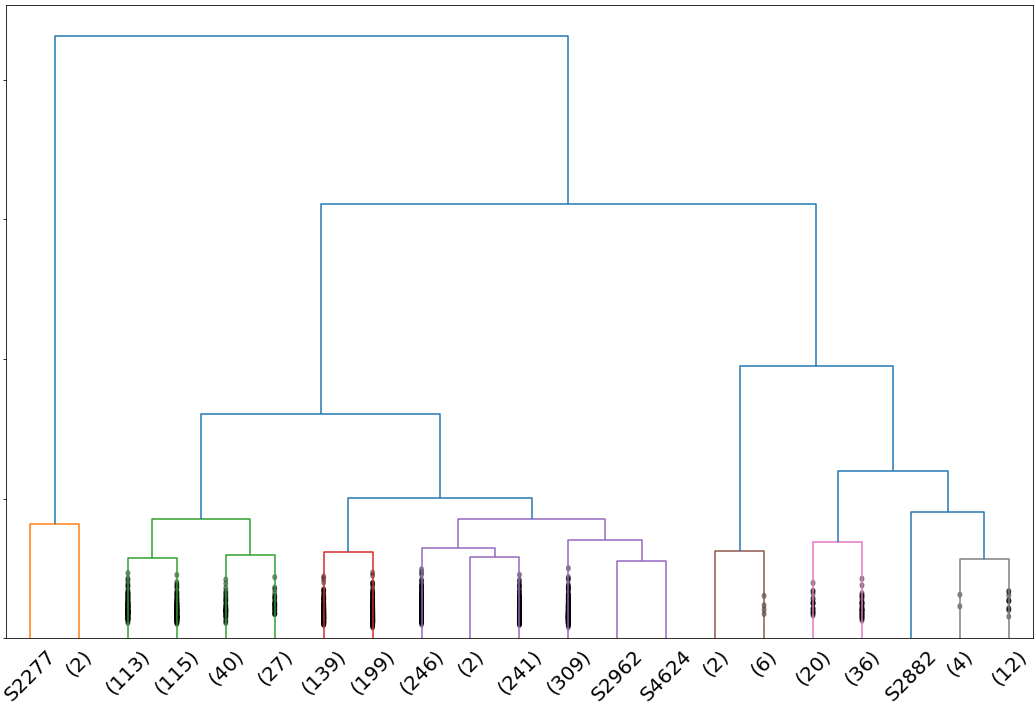
\includegraphics[width=.49\textwidth]{img/anomalies/anomalies_H_dendrogramme.png}
   \caption{Dendrogram associated to a complete-linkage hierarchical clustering of the persistence diagrams of men point clouds with the Wasserstein distance. Clusters composed of one individual are presented without parentheses.}
   \label{fig:anomaly_dendrogram_H}
\end{figure}

\begin{figure}[H]
    \centering
    \subfigure[\tt S2277]{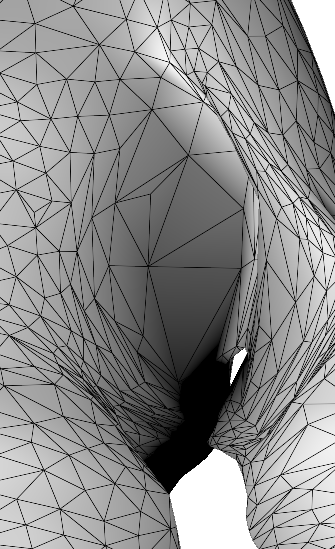
\includegraphics[height=.088\textheight]{img/anomalies/anomalies_H_822_2.png}}\;
    \subfigure[\tt S2962]{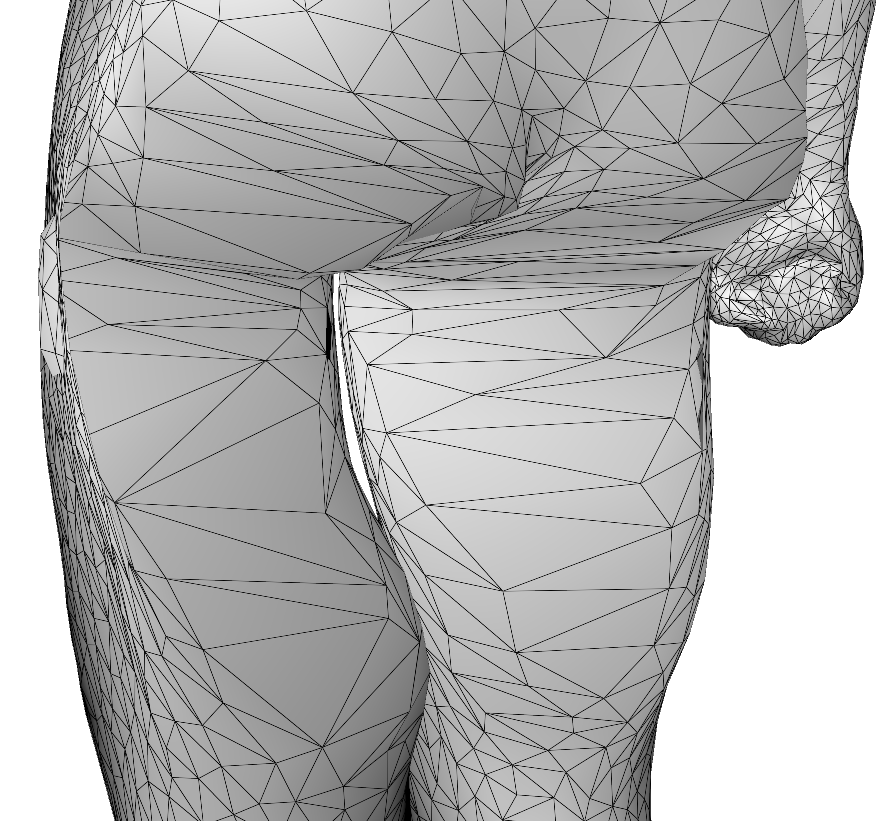
\includegraphics[height=.088\textheight]{img/anomalies/anomalies_H_1076_2.png}}\;
    \subfigure[\tt S4624]{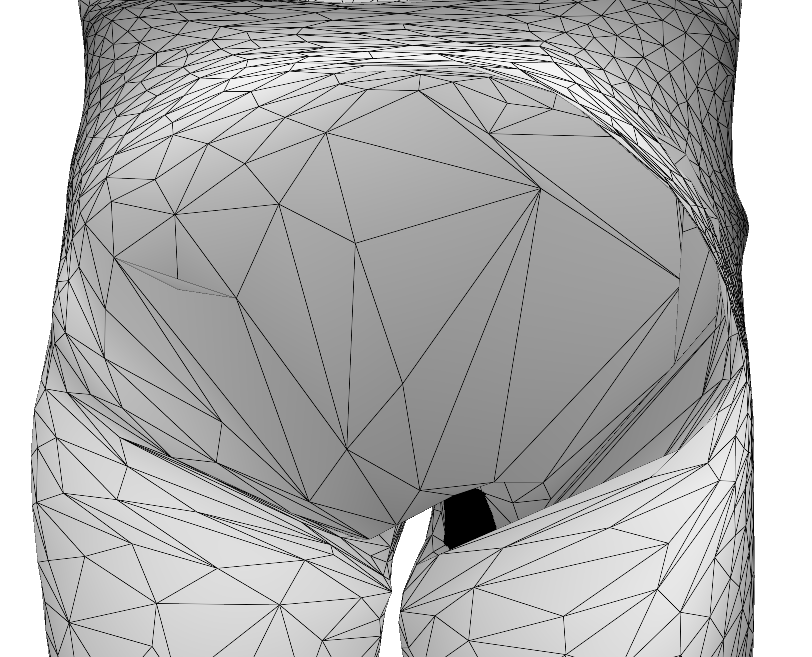
\includegraphics[height=.088\textheight]{img/anomalies/anomalies_H_1438_2.png}}\;
    \subfigure[\tt S2882]{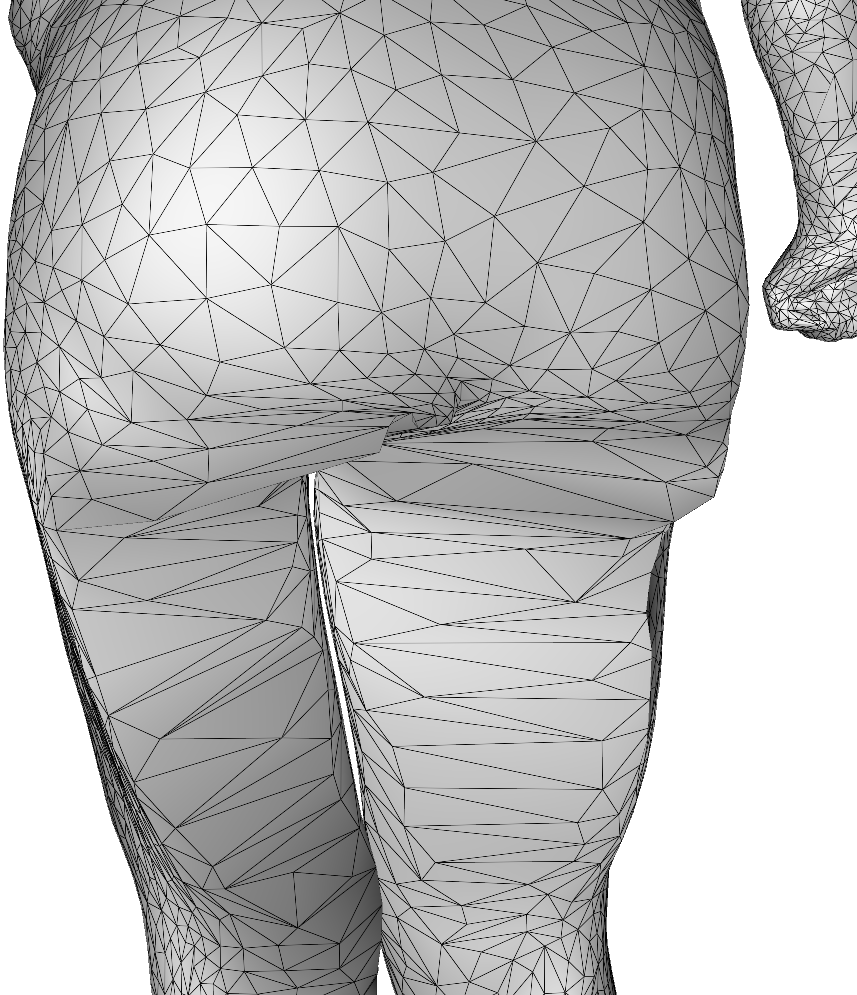
\includegraphics[height=.088\textheight]{img/anomalies/anomalies_H_1034_2.png}}
    \caption{Anomalies of men scans detected by complete-linkage hierarchical clustering of persistence diagrams.}
    \label{fig:anomaly_scans_H}
\end{figure}

To illustrate that anomalies are detected by persistence, we analyse the persistence diagram of Figure \ref{fig:anomaly_DP_1076_H} which corresponds to the individual {\tt S2962}.
\vspace{0.2cm}

Its three $H_2$ homologies $n^{\circ}3,5,6$ are particularly distinguished and can be seen at birth and death in Figure \ref{fig:anomaly_homologies_1076_H}. Homologies $H_2$ number $3$ and $5$ correspond to the right and left leg respectively while the number 6 corresponds to the torso and is the principal $H_2$-homology.

For normal scans, the principal $H_2$-homology aggregates also legs. Because of the misplaced points and the holes on the point cloud, legs homologies are separated from the principal $H_2$-homology which starts later than normally.

\begin{figure}[H]
    \centering
    \subfigure[Persistence diagram]{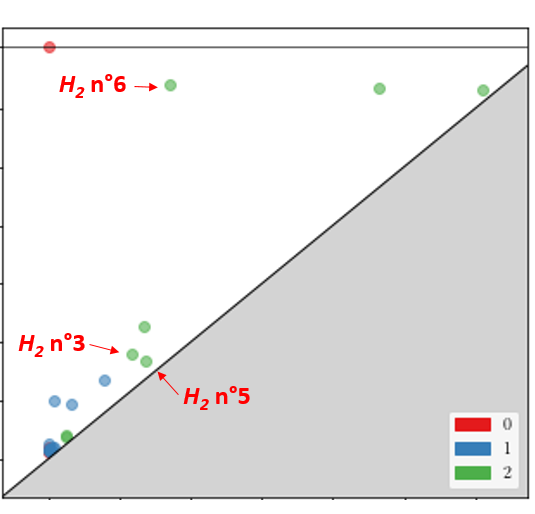
\includegraphics[height=.17\textheight]{img/anomalies/anomalies_H_DP_1076_d.png}}
    \subfigure[Persistence barcode]{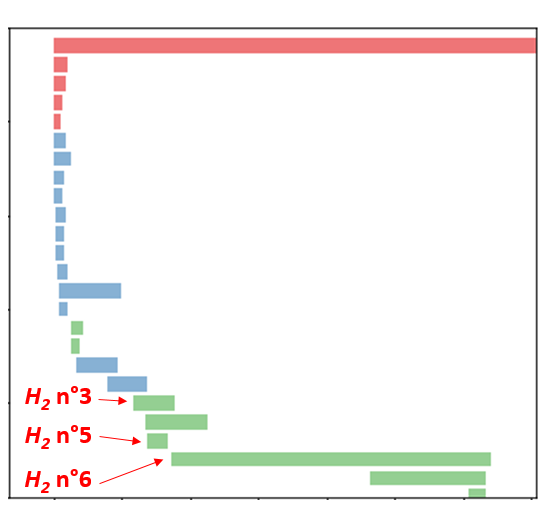
\includegraphics[height=.17\textheight]{img/anomalies/anomalies_H_DP_1076_b.png}}
    \caption{Persistence diagram and barcode of the anomaly of scan {\tt S2962}. Three particular homologies reflecting the anomaly are highlighted.}
    \label{fig:anomaly_DP_1076_H}
\end{figure}

\begin{figure}[H]
    \centering
    \subfigure[$H_2$ n°3]{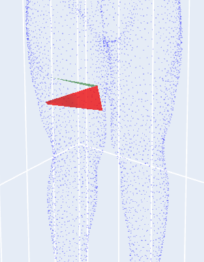
\includegraphics[height=.14\textheight]{img/anomalies/anomalies_H2_n3.png}}\;
    \subfigure[$H_2$ n°5]{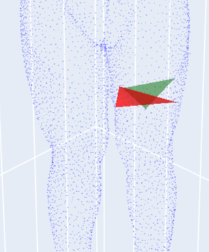
\includegraphics[height=.14\textheight]{img/anomalies/anomalies_H2_n5.png}}\; 
    \subfigure[$H_2$ n°6]{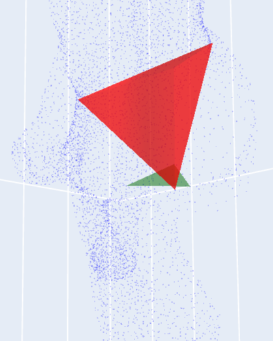
\includegraphics[height=.14\textheight]{img/anomalies/anomalies_H2_n6.png}}
    \caption{Three abnormal homologies at birth and death of the defective scan {\tt S2962}.}
    \label{fig:anomaly_homologies_1076_H}
\end{figure}

For women the best truncation range is $[23,37]$ where the criteria gives $87.5 \%$ : $100 \%$ of isolated individuals are anomalies and $75 \%$ of anomalies are detected. Figure \ref{fig:anomaly_dendrogram_F} shows the dendrogram for women point clouds truncated at $23$ clusters where the $3$ isolated individuals are anomalies as shown in Figure \ref{fig:anomaly_scans_F}.

\begin{figure}[H]
  \centering
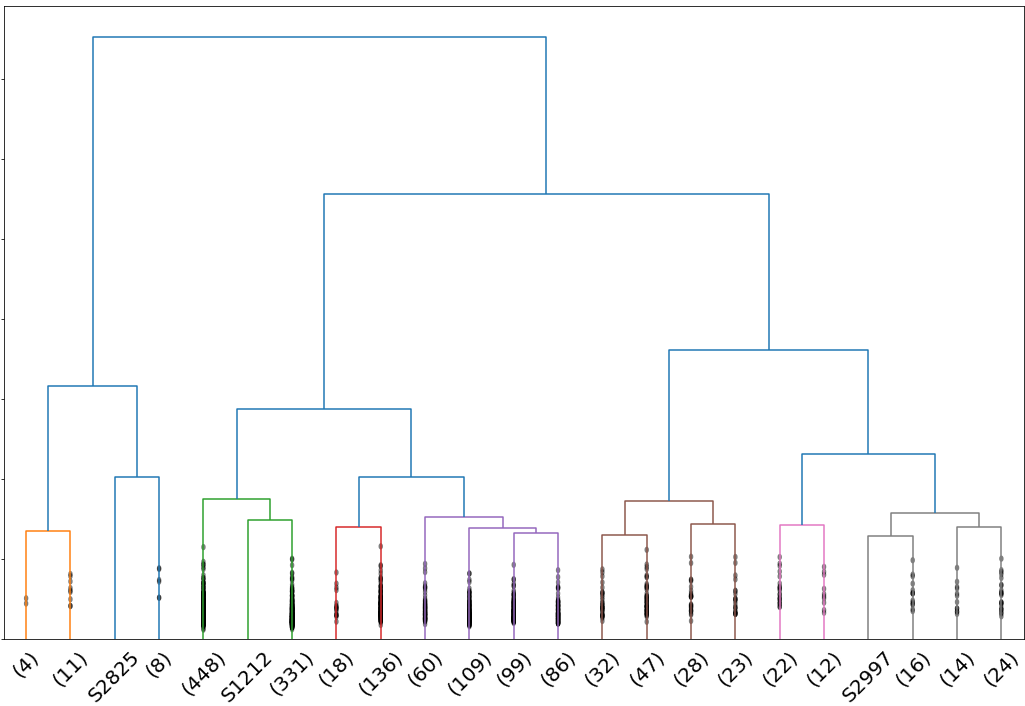
\includegraphics[width=.49\textwidth]{img/anomalies/anomalies_F_dendrogramme.png}
   \caption{Dendrogram associated to a complete-linkage hierarchical clustering of the persistence diagrams of women point clouds with the Wasserstein distance.}
   \label{fig:anomaly_dendrogram_F}
\end{figure}

\begin{figure}[H]
    \centering
    \subfigure[\tt S2825]{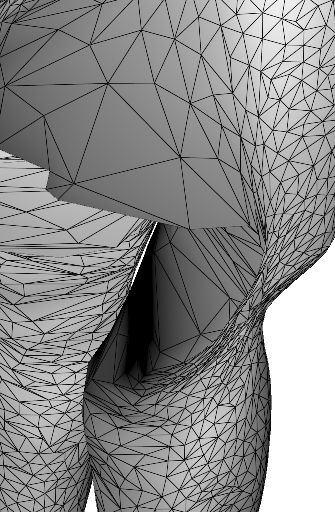
\includegraphics[height=.12\textheight]{img/anomalies/anomalies_F_2825_2.png}}\;
    \subfigure[\tt S1212]{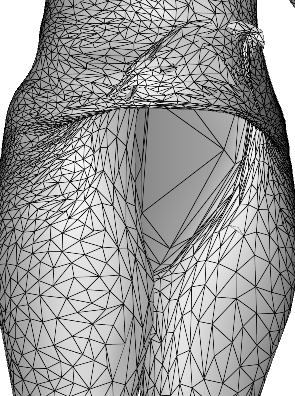
\includegraphics[height=.12\textheight]{img/anomalies/anomalies_F_1212_2.png}}\;
    \subfigure[\tt S2997]{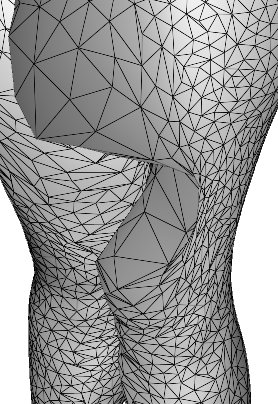
\includegraphics[height=.12\textheight]{img/anomalies/anomalies_F_2997_2.png}}
    \caption{Anomalies of women scans detected by complete-linkage hierarchical clustering of persistence diagrams.}
    \label{fig:anomaly_scans_F}
\end{figure}

\section{Gender discrimination index} \label{sec:GDI}

In this section we analyse if clustering algorithms on persistence diagrams and silhouettes give groups separating men from women scans by changing the number of clusters. To this end we use persistence diagrams or silhouettes, restricted to trunks of point clouds or not.

Let $P_m(C)$ and $P_f(C)$ be respectively the proportions of men and women in a cluster $C$. We have

\begin{equation*}
    P_m(C)=\frac{n_m(C)}{s(C)}, \qquad P_f(C)=\frac{n_f(C)}{s(C)}
\end{equation*}
where $n_m(C)$ is the number of men in $C$, $n_f(C)$ is the number of women in $C$ and $s(C)$ is the size of $C$. To mesure the quality of a clustering $\mathcal{C}$ of a set of mixed men and women diagrams or silhouettes $D_{MF}$, we introduce a gender discrimination index (GDI) defined by
\begin{equation*}
    GDI(\mathcal{C})=\frac{2}{s(D_{MF})}\sum\limits_{k=1}^K s(C_k)\left|P_m(C_k)-\frac{1}{2}\right|
\end{equation*}
where $K$ is the number of clusters of $\mathcal{C}$, $C_k$ are the clusters of $\mathcal{C}$ and $s(D_{MF})$ is the number of elements in $D_{MF}$. Thus, the better the clustering $\mathcal{C}$ separates men from women, the closer $GDI(\mathcal{C})$ is to 1 ; and the worse it is, the closer $GDI(\mathcal{C})$ is to 0. We can consider that a clustering is satisfactory to separate men from women if its GDI is greater or equal to $\frac{1}{2}$.

\subsection{Evolution of the GDI score as a function of the number of clusters}

In this section, we will observe the ability of different clustering methods to separate male from female persistence diagrams or silhouettes.

We use a matrix of Wasserstein distances between diagrams to perform hierarchical clustering with complete and Ward's linkage methods \cite{W63} as well as K-Medoids clustering with PAM (Partitioning Around Medoids) algorithm \cite{KR90}. The notion of barycenter between persistence diagrams is delicate \cite{MMH11}, \cite{TMMH12} but we can use the Ward-linkage method with the Lance-Williams algorithm \cite{LW67}.

\begin{figure}[H]
    \centering
    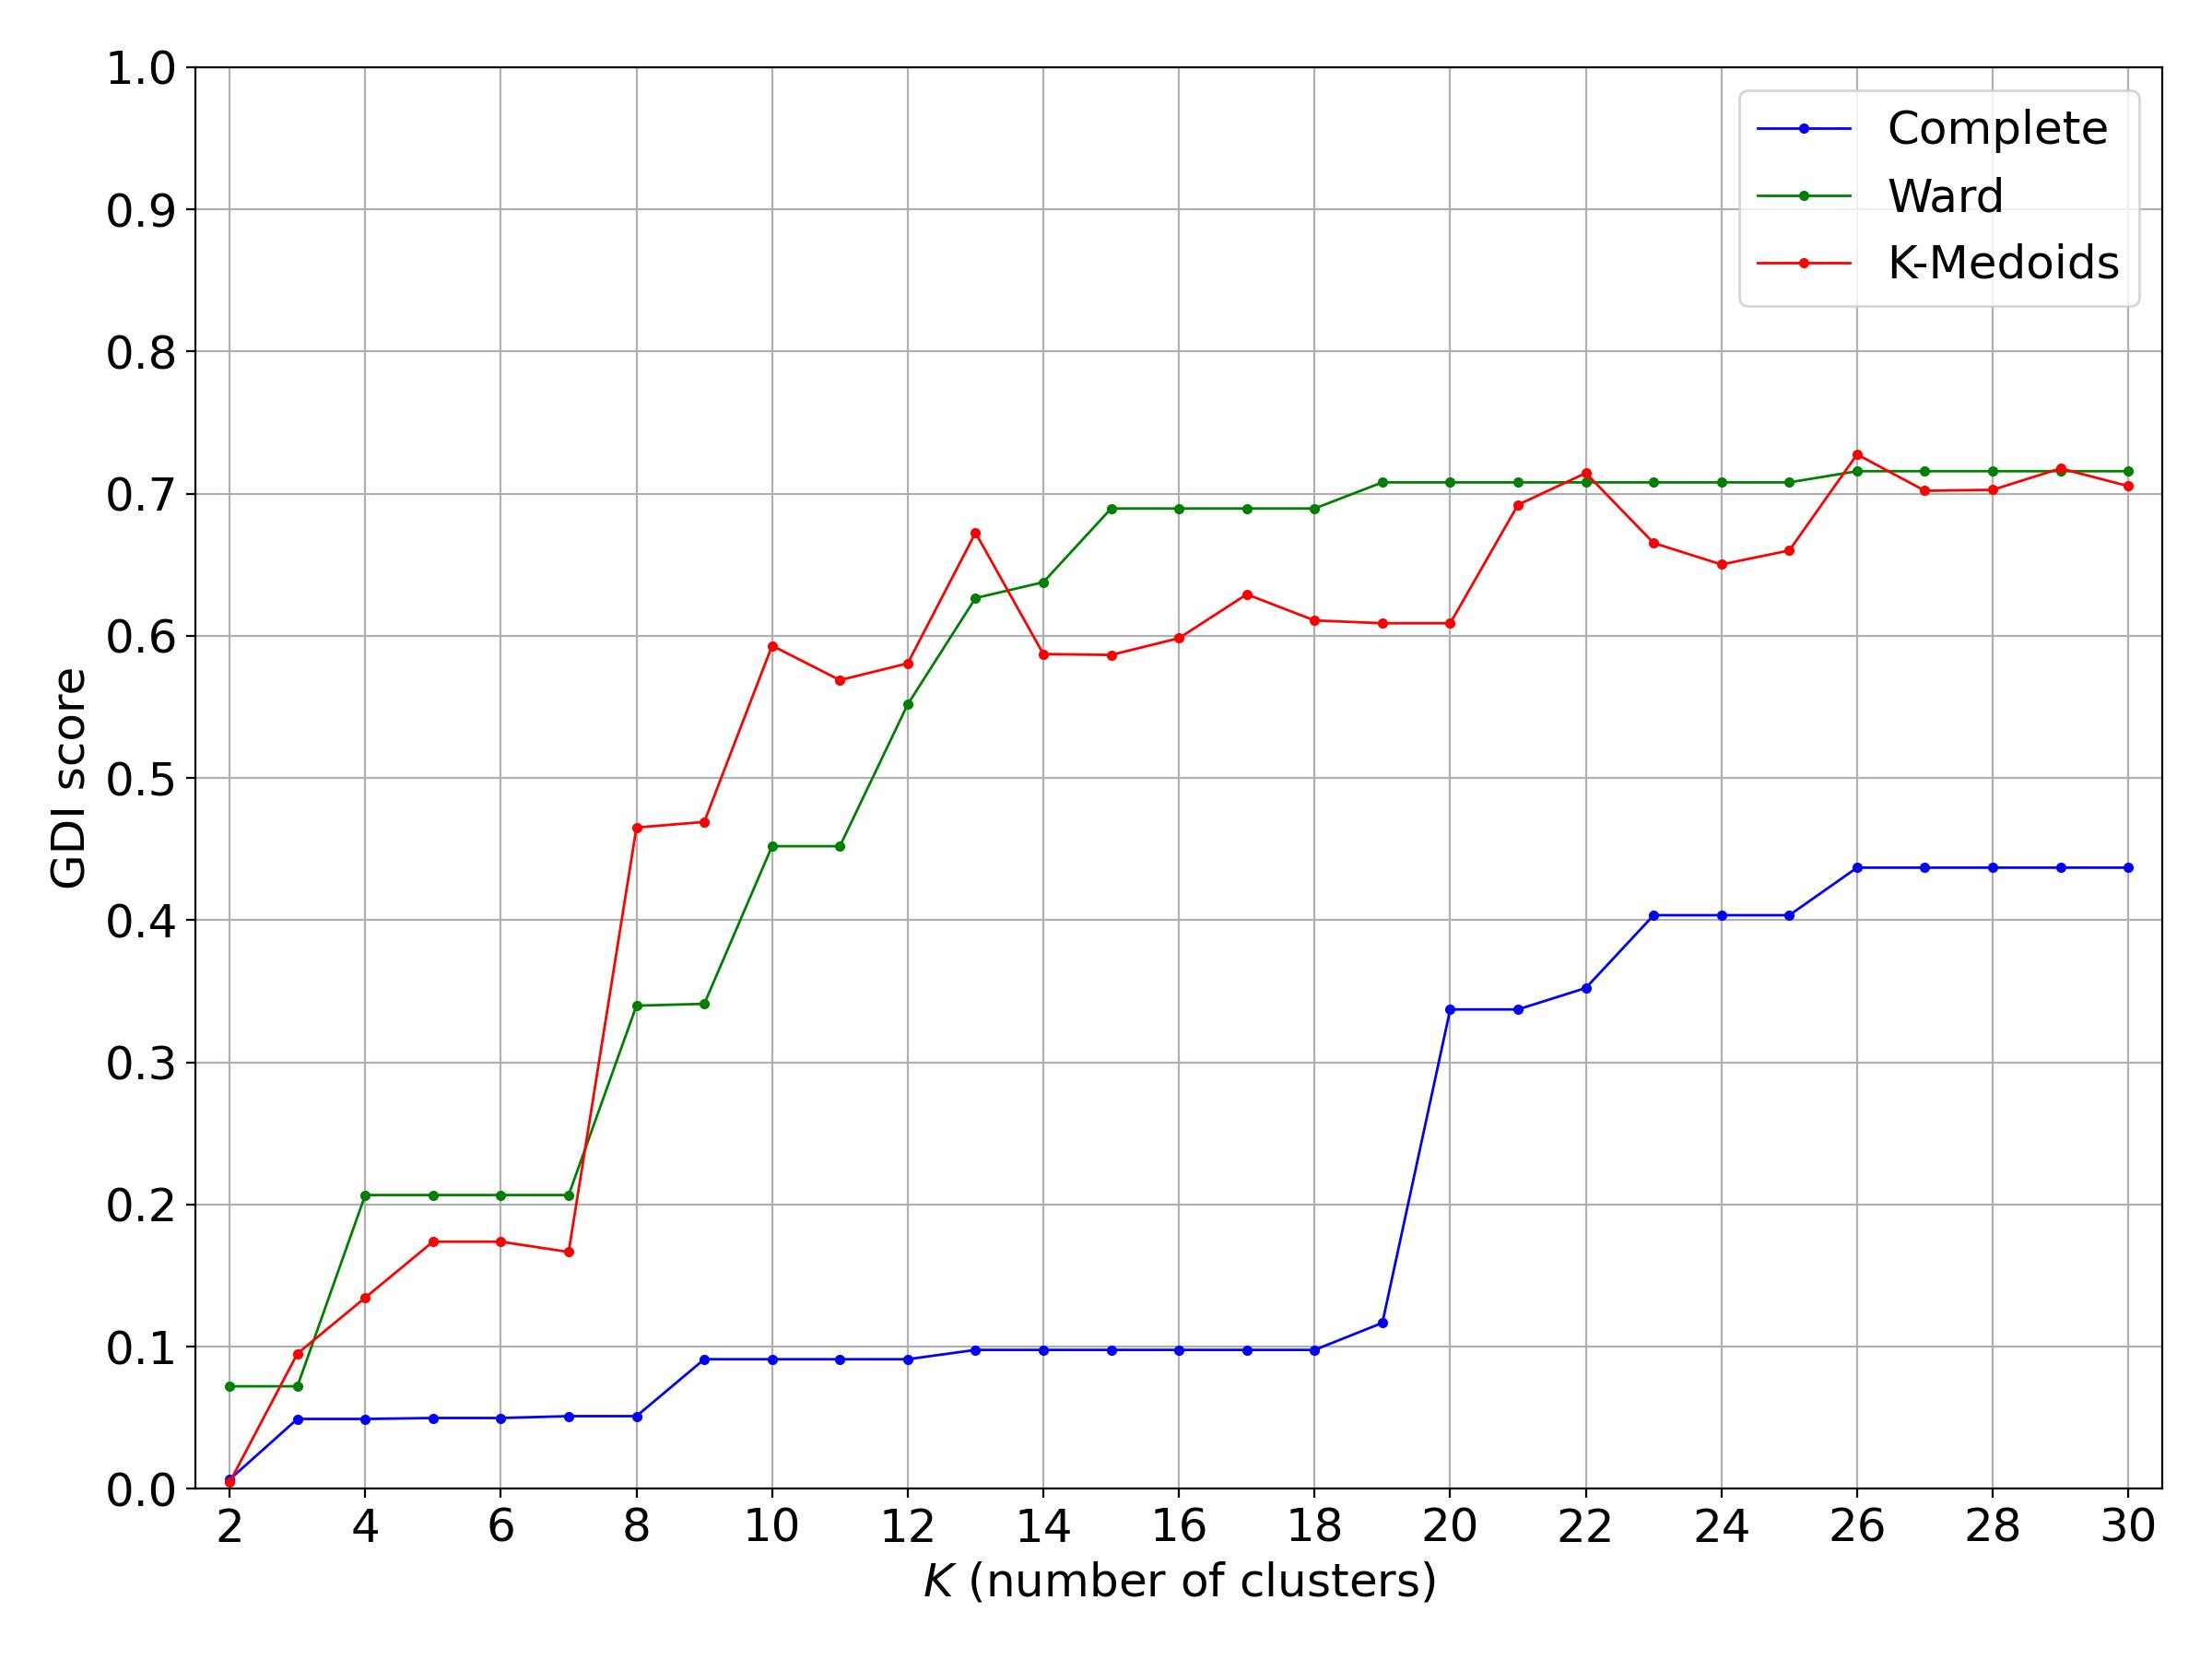
\includegraphics[width=.49\textwidth]{img/GDI/MFGDI.jpg}
    \caption{GDI score evolution of various clustering algorithms on the persistence diagrams with Wasserstein distance.}
    \label{fig:gdi_Wasserstein}
\end{figure}

As shown in Figure \ref{fig:gdi_Wasserstein}, hierarchical clustering with the complete-linkage method does not differentiate correctly between female and male scans. However, the K-Medoids clustering has a correct GDI score for more than 10 clusters and becomes good on some occasions for more than 13 clusters. The Ward-linkage hierarchical clustering has a correct GDI score for more than 12 clusters and becomes good for more than 19 clusters
\vspace{0.2cm}

We now use vectors obtained from the silhouettes associated to the persistence diagrams of scans on which we perform a Ward-linkage hierarchical clustering as well as a K-Means clustering and a K-Medoids clustering with PAM algorithm. This time, these three clustering algorithms give very good GDI score, see Figure \ref{fig:gdi_silhouette}.

\begin{figure}[!ht]
    \centering
    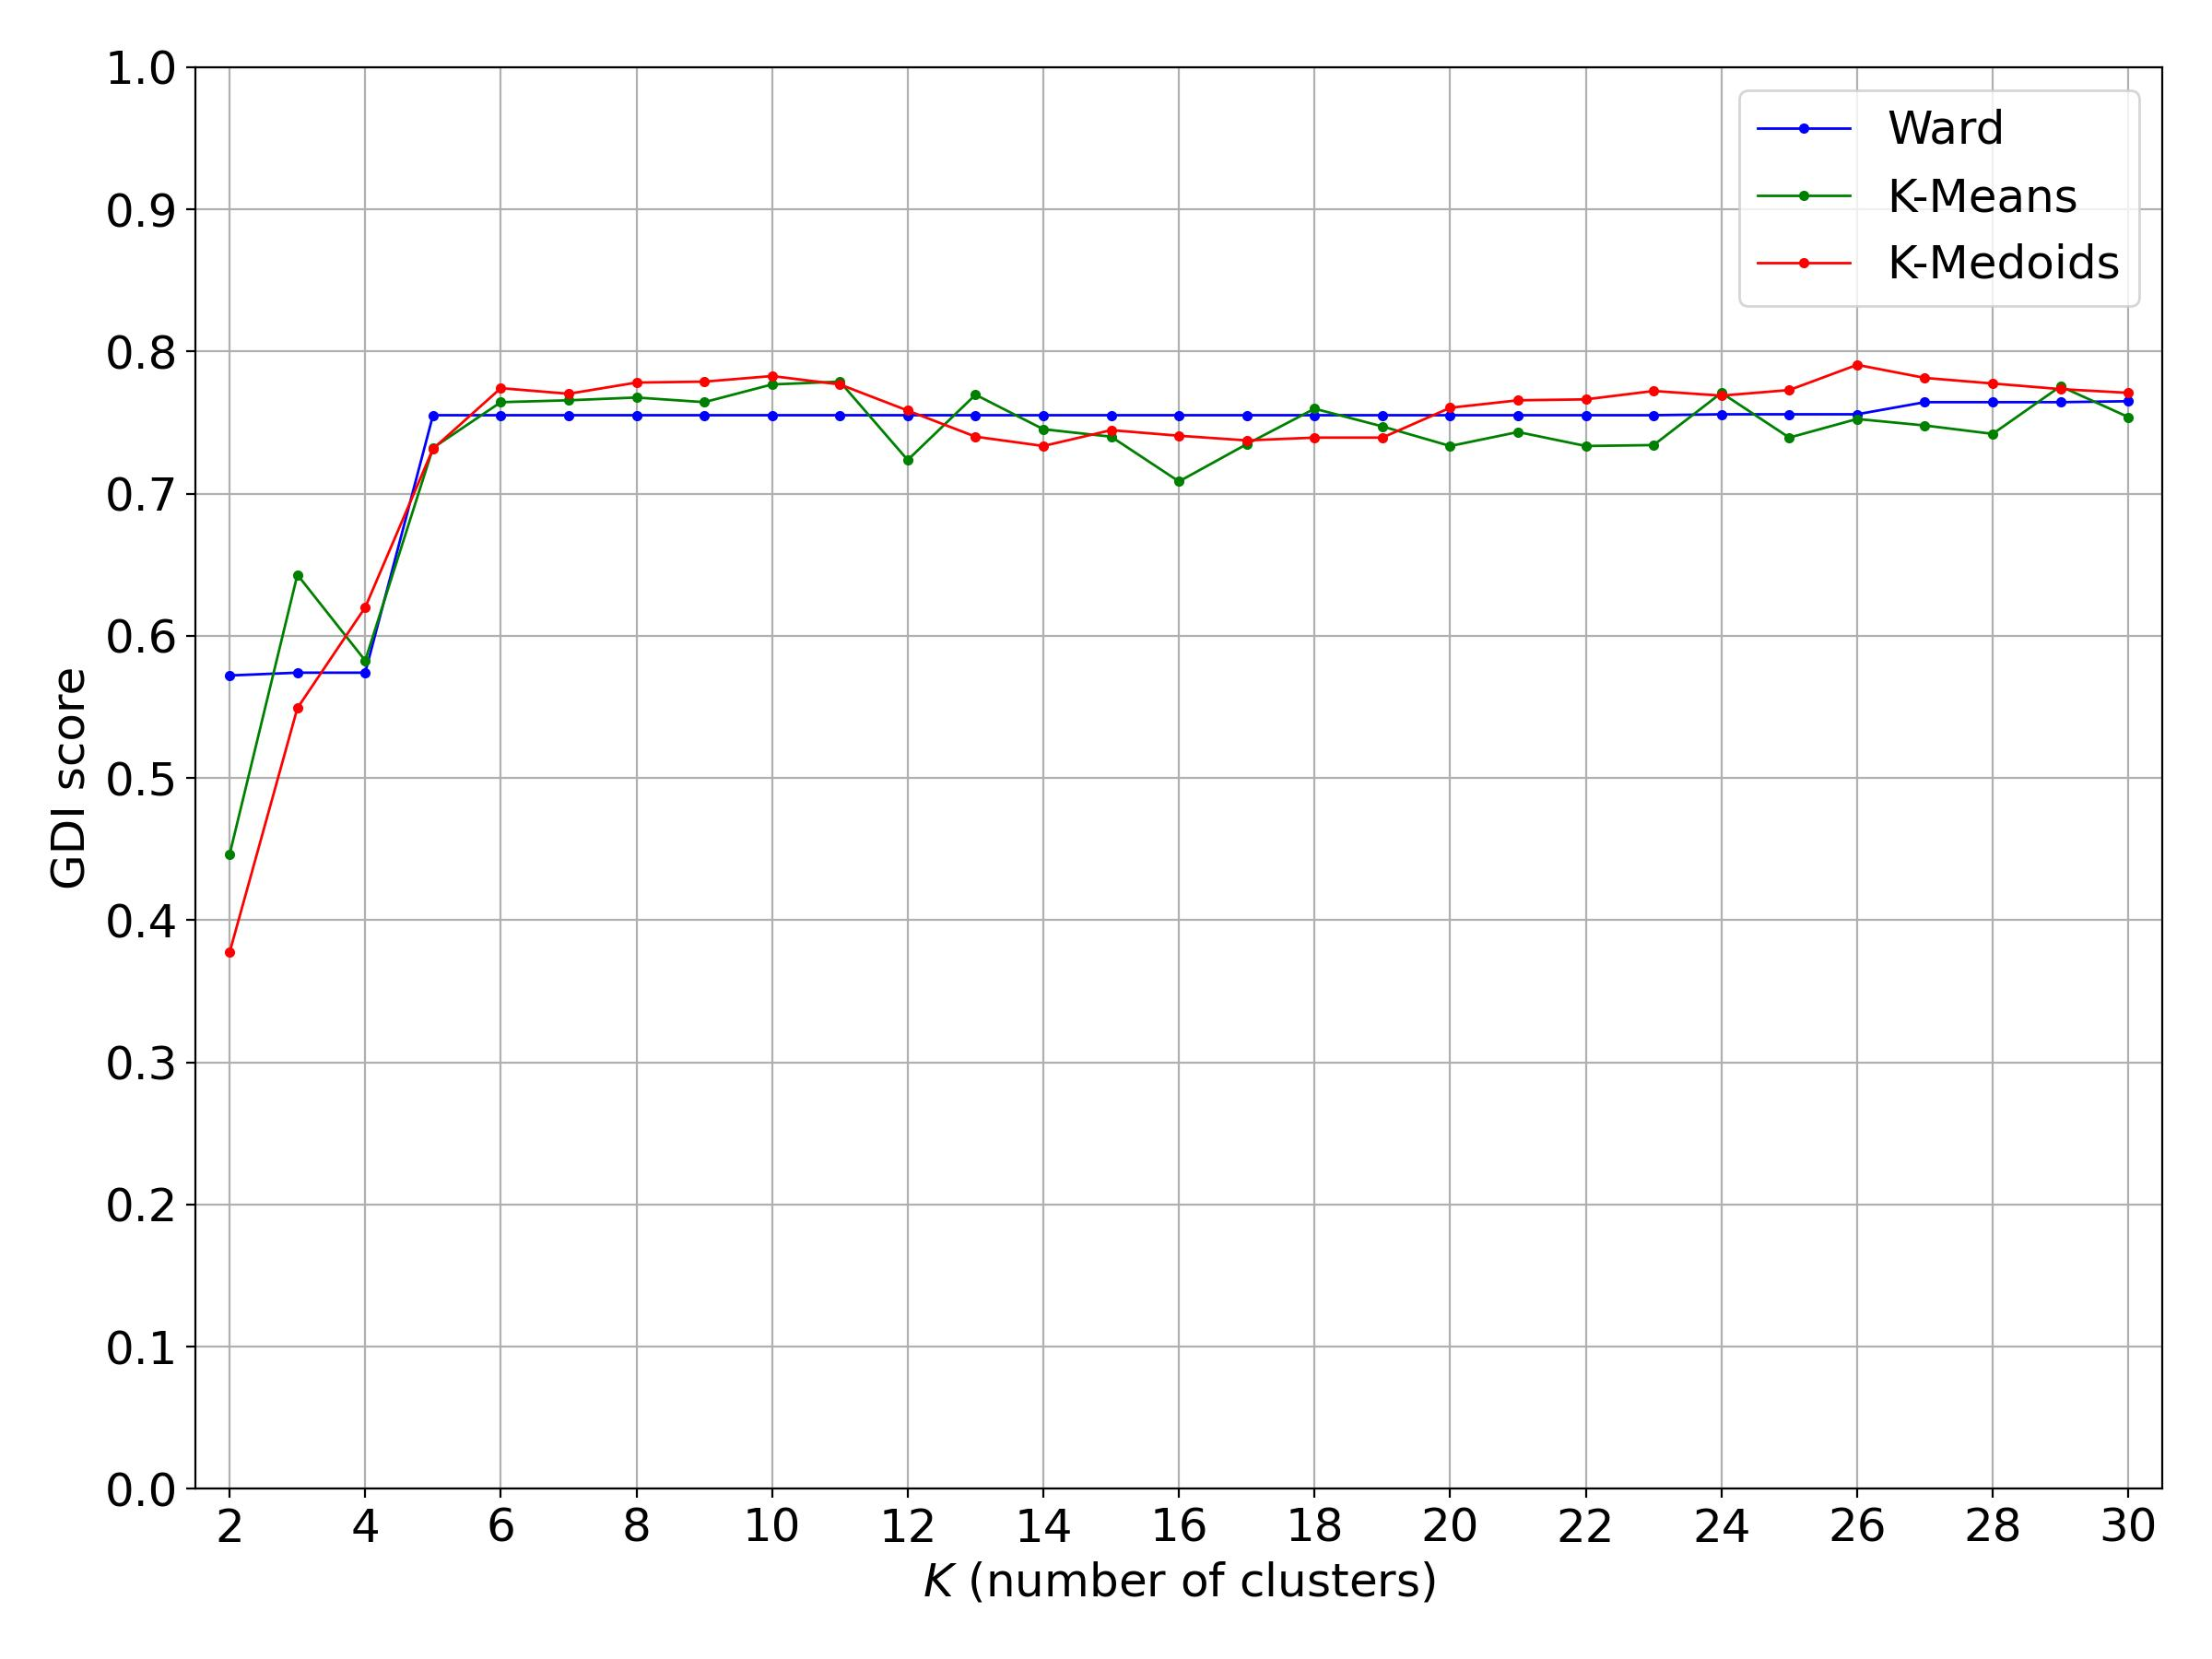
\includegraphics[width=.49\textwidth]{img/GDI/MFsGDI.jpg}
    \caption{GDI score evolution of various clustering algorithms on the persistence silhouettes.}
    \label{fig:gdi_silhouette}
\end{figure}

\subsection{Restriction to trunks}

When constructing the silhouettes, we used a weighting that tended to favour the $H_2$ homologies corresponding to the trunks of the subjects, so the question then arises as to whether we would obtain better results by using only the points corresponding to the trunk of the body. To this end we have developed an algorithm to isolate the points corresponding to the trunk of an individual, see Figure \ref{fig:full+trunk}.

\begin{figure}[H]
    \centering
    \subfigure[Full body]{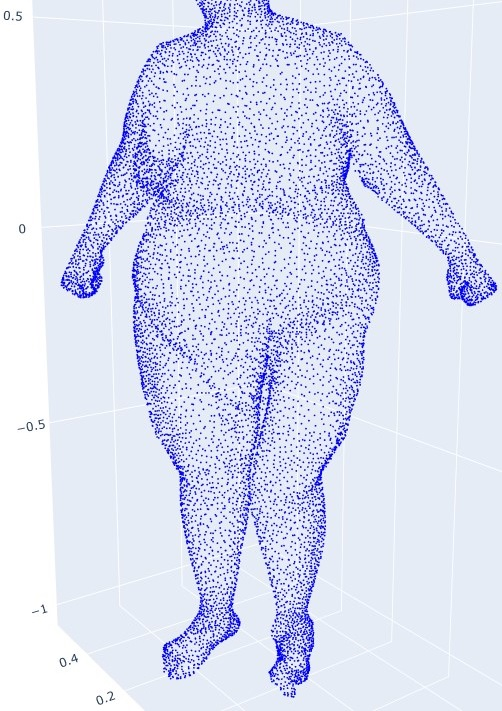
\includegraphics[height=.24\textheight]{img/Trunk/Trunk_F1039_before.jpg}}\;
    \subfigure[Trunk]{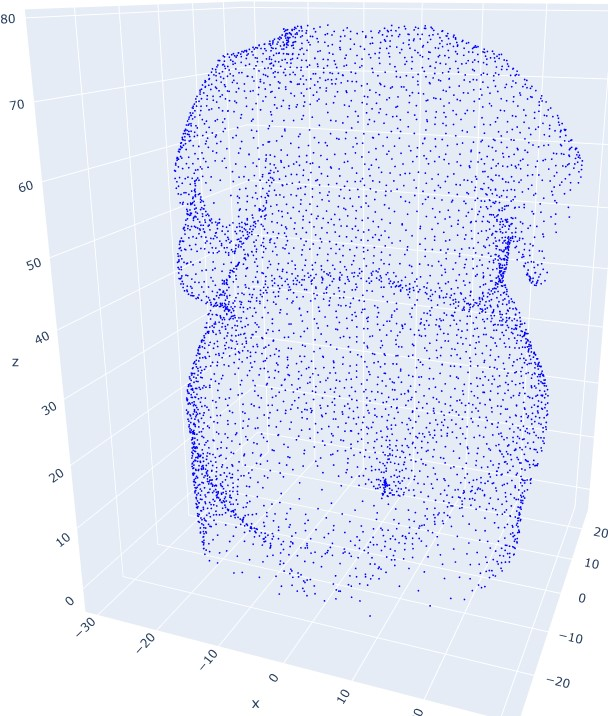
\includegraphics[width=.16\textheight]{img/Trunk/Trunk_F1039_after.jpg}}
    \caption{An individual and its isolated trunk.}
    \label{fig:full+trunk}
\end{figure}

We now compare the clustering results using a Wasserstein distance matrix applied to the whole body and applied to the trunk.

From the curves in Figure \ref{Fig:gdi_W_BT} and the average GDI scores of Table \ref{Tab:gdi_W_BT}, it appears that for clustering algorithms based on Wasserstein distances between persistence diagrams, it is not worth restricting to trunk points.

\begin{table}[H]
	\centering
	\begin{tabular}{|c|c|c|c|}
		\hline
				&Complete	&Ward	&K-Medoids	\\ \hline
		Body	&0.2		&0.54	&0.526		\\ \hline
		Trunk	&0.21		&0.553	&0.582		\\ \hline
	\end{tabular}
		\caption{Average GDI scores on the persistence diagrams of the whole body and the trunk with the Wasserstein distance.}
	\label{Tab:gdi_W_BT}
\end{table}

\begin{figure}[H]
	\centering
	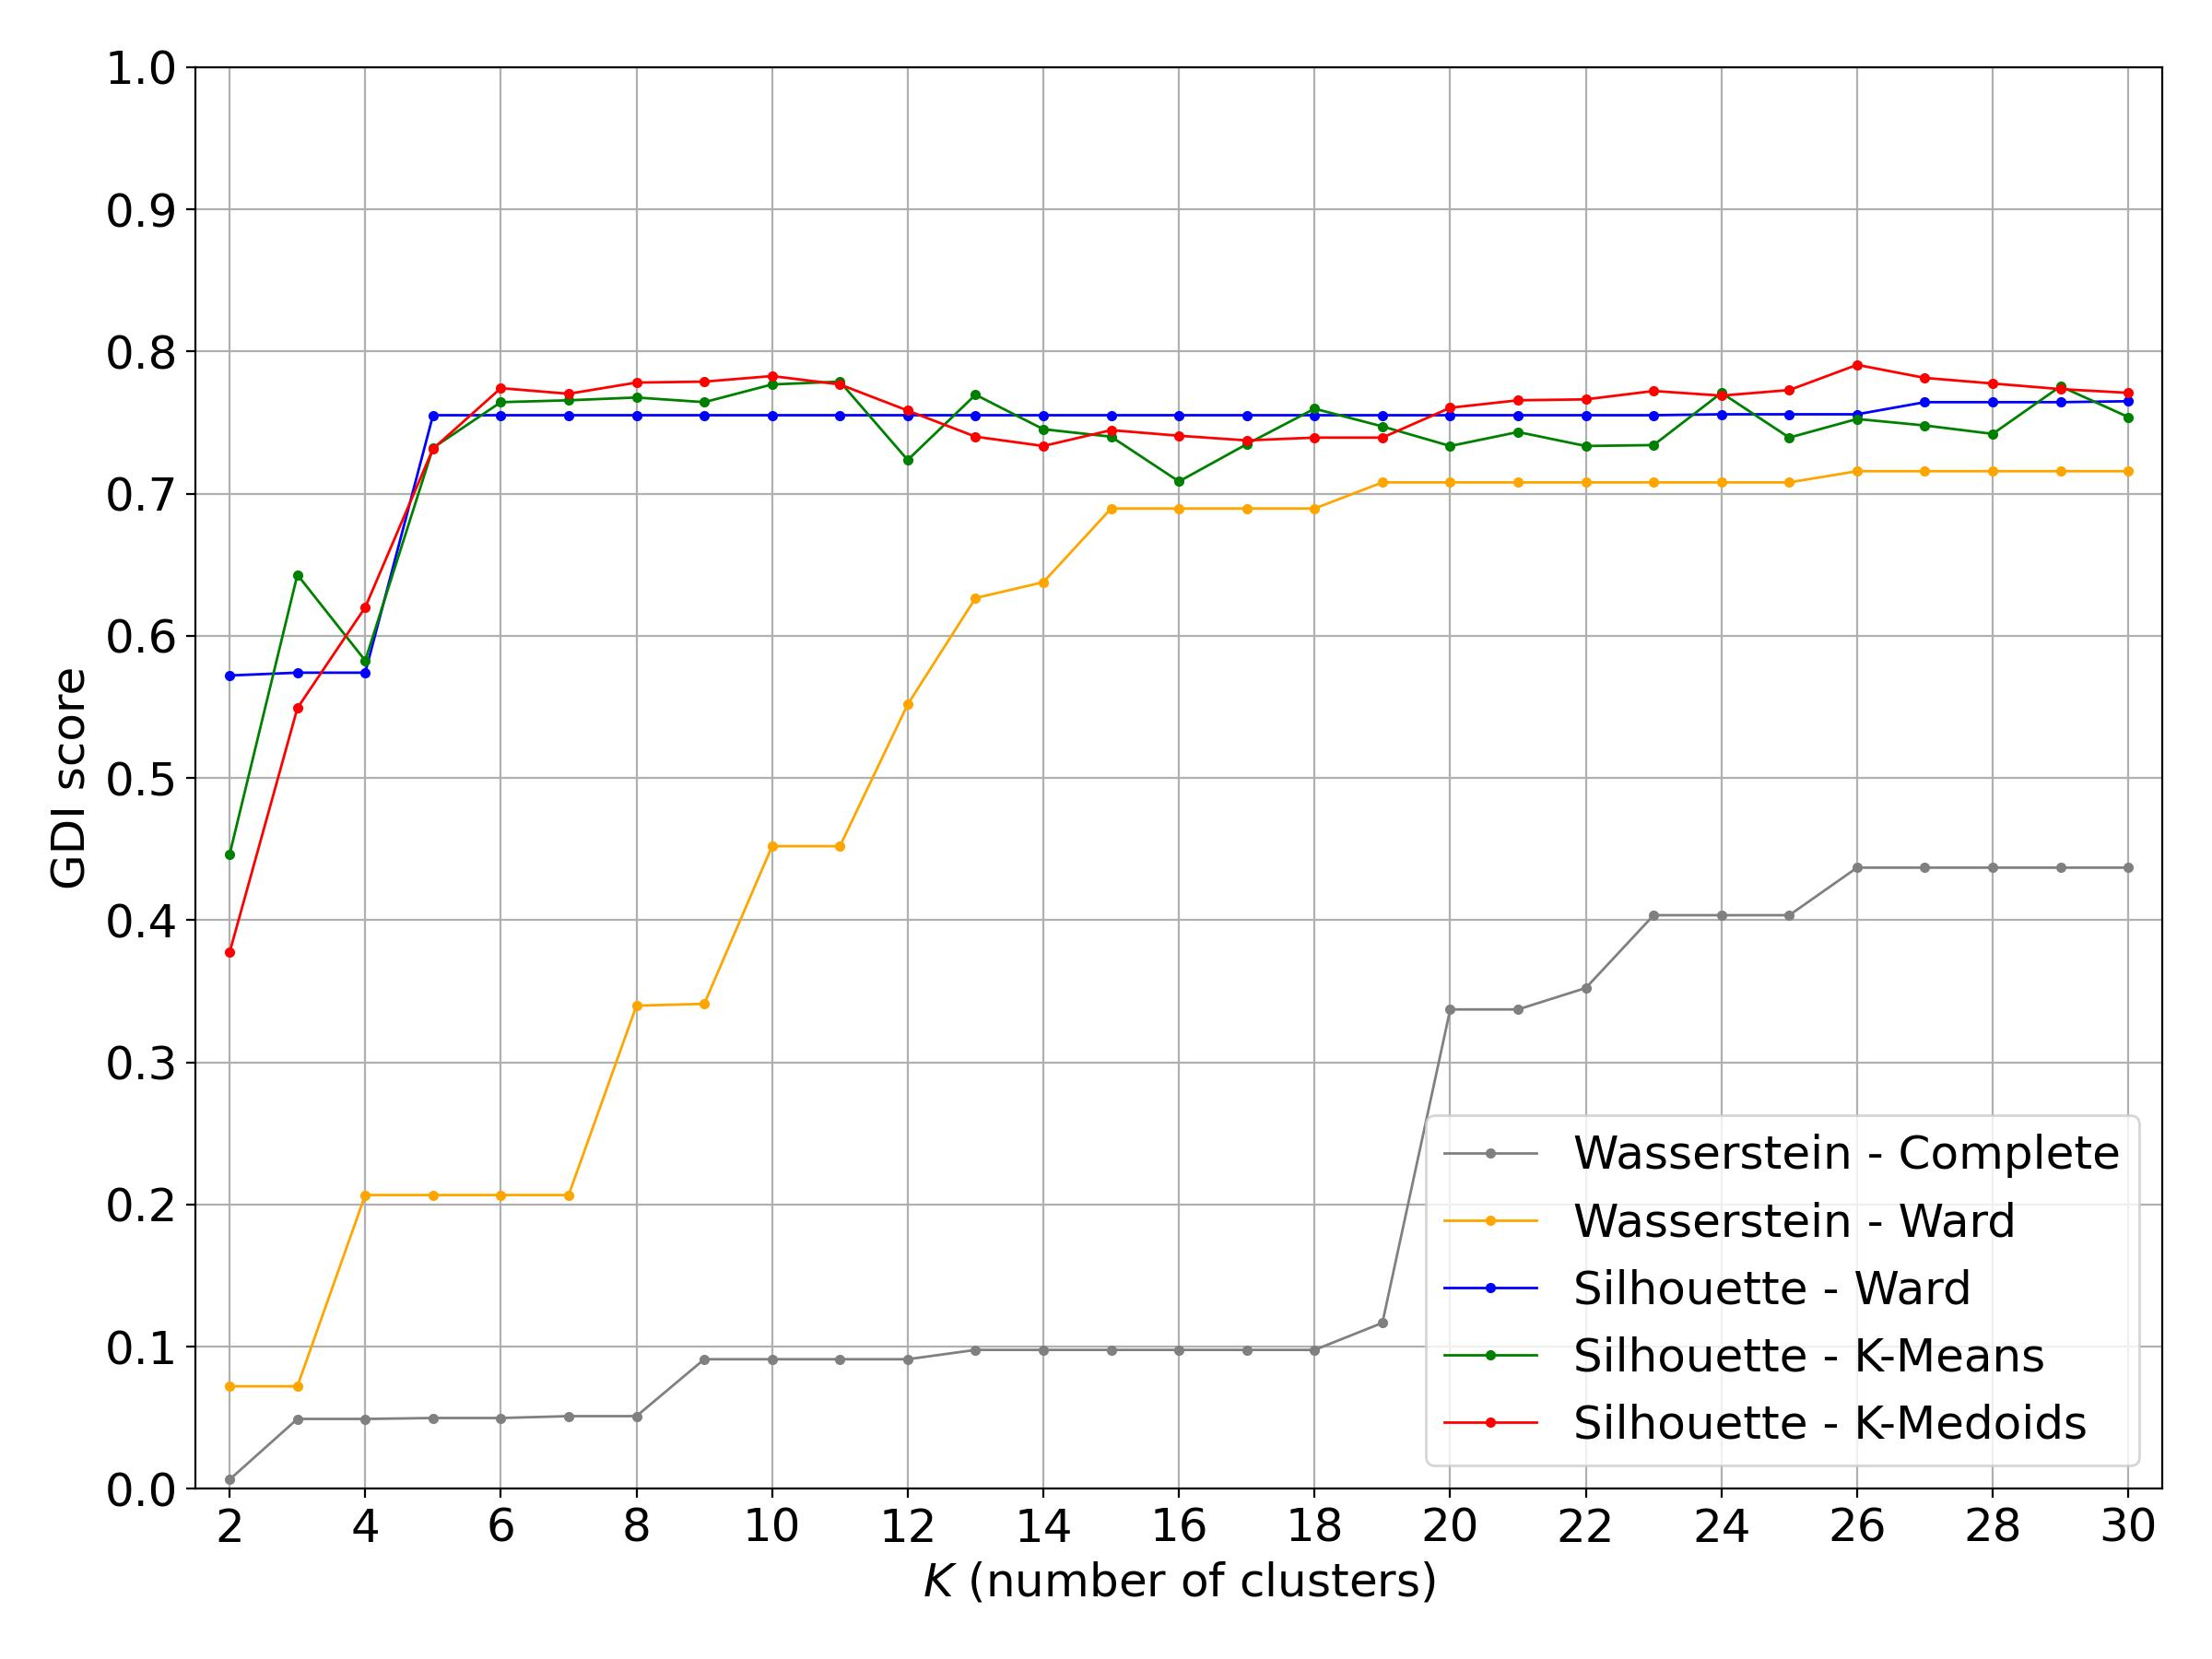
\includegraphics[width=.49\textwidth]{img/GDI/TWMFGDI}
	\caption{Comparison of GDI score on the persistence diagrams of the whole body and the trunk with the Wasserstein distance.}
	\label{Fig:gdi_W_BT}
\end{figure}

We now compare the results of clustering algorithms using the vectors obtained from the persistence silhouettes applied to the whole body and applied to the trunk.

\begin{table}[H]
	\centering
	\begin{tabular}{|c|c|c|c|}
		\hline
		&Ward	&K-Means	&K-Medoids \\ \hline
		Body	&0.738		&0.73	&0.737 \\ \hline
		Trunk	&0.765		&0.767	&0.827 \\ \hline
	\end{tabular}
		\caption{Average GDI scores on the persistence silhouettes of the whole body and the trunk.}
	\label{Tab:gdi_S_BT}
\end{table}

\begin{figure}[H]
	\centering
	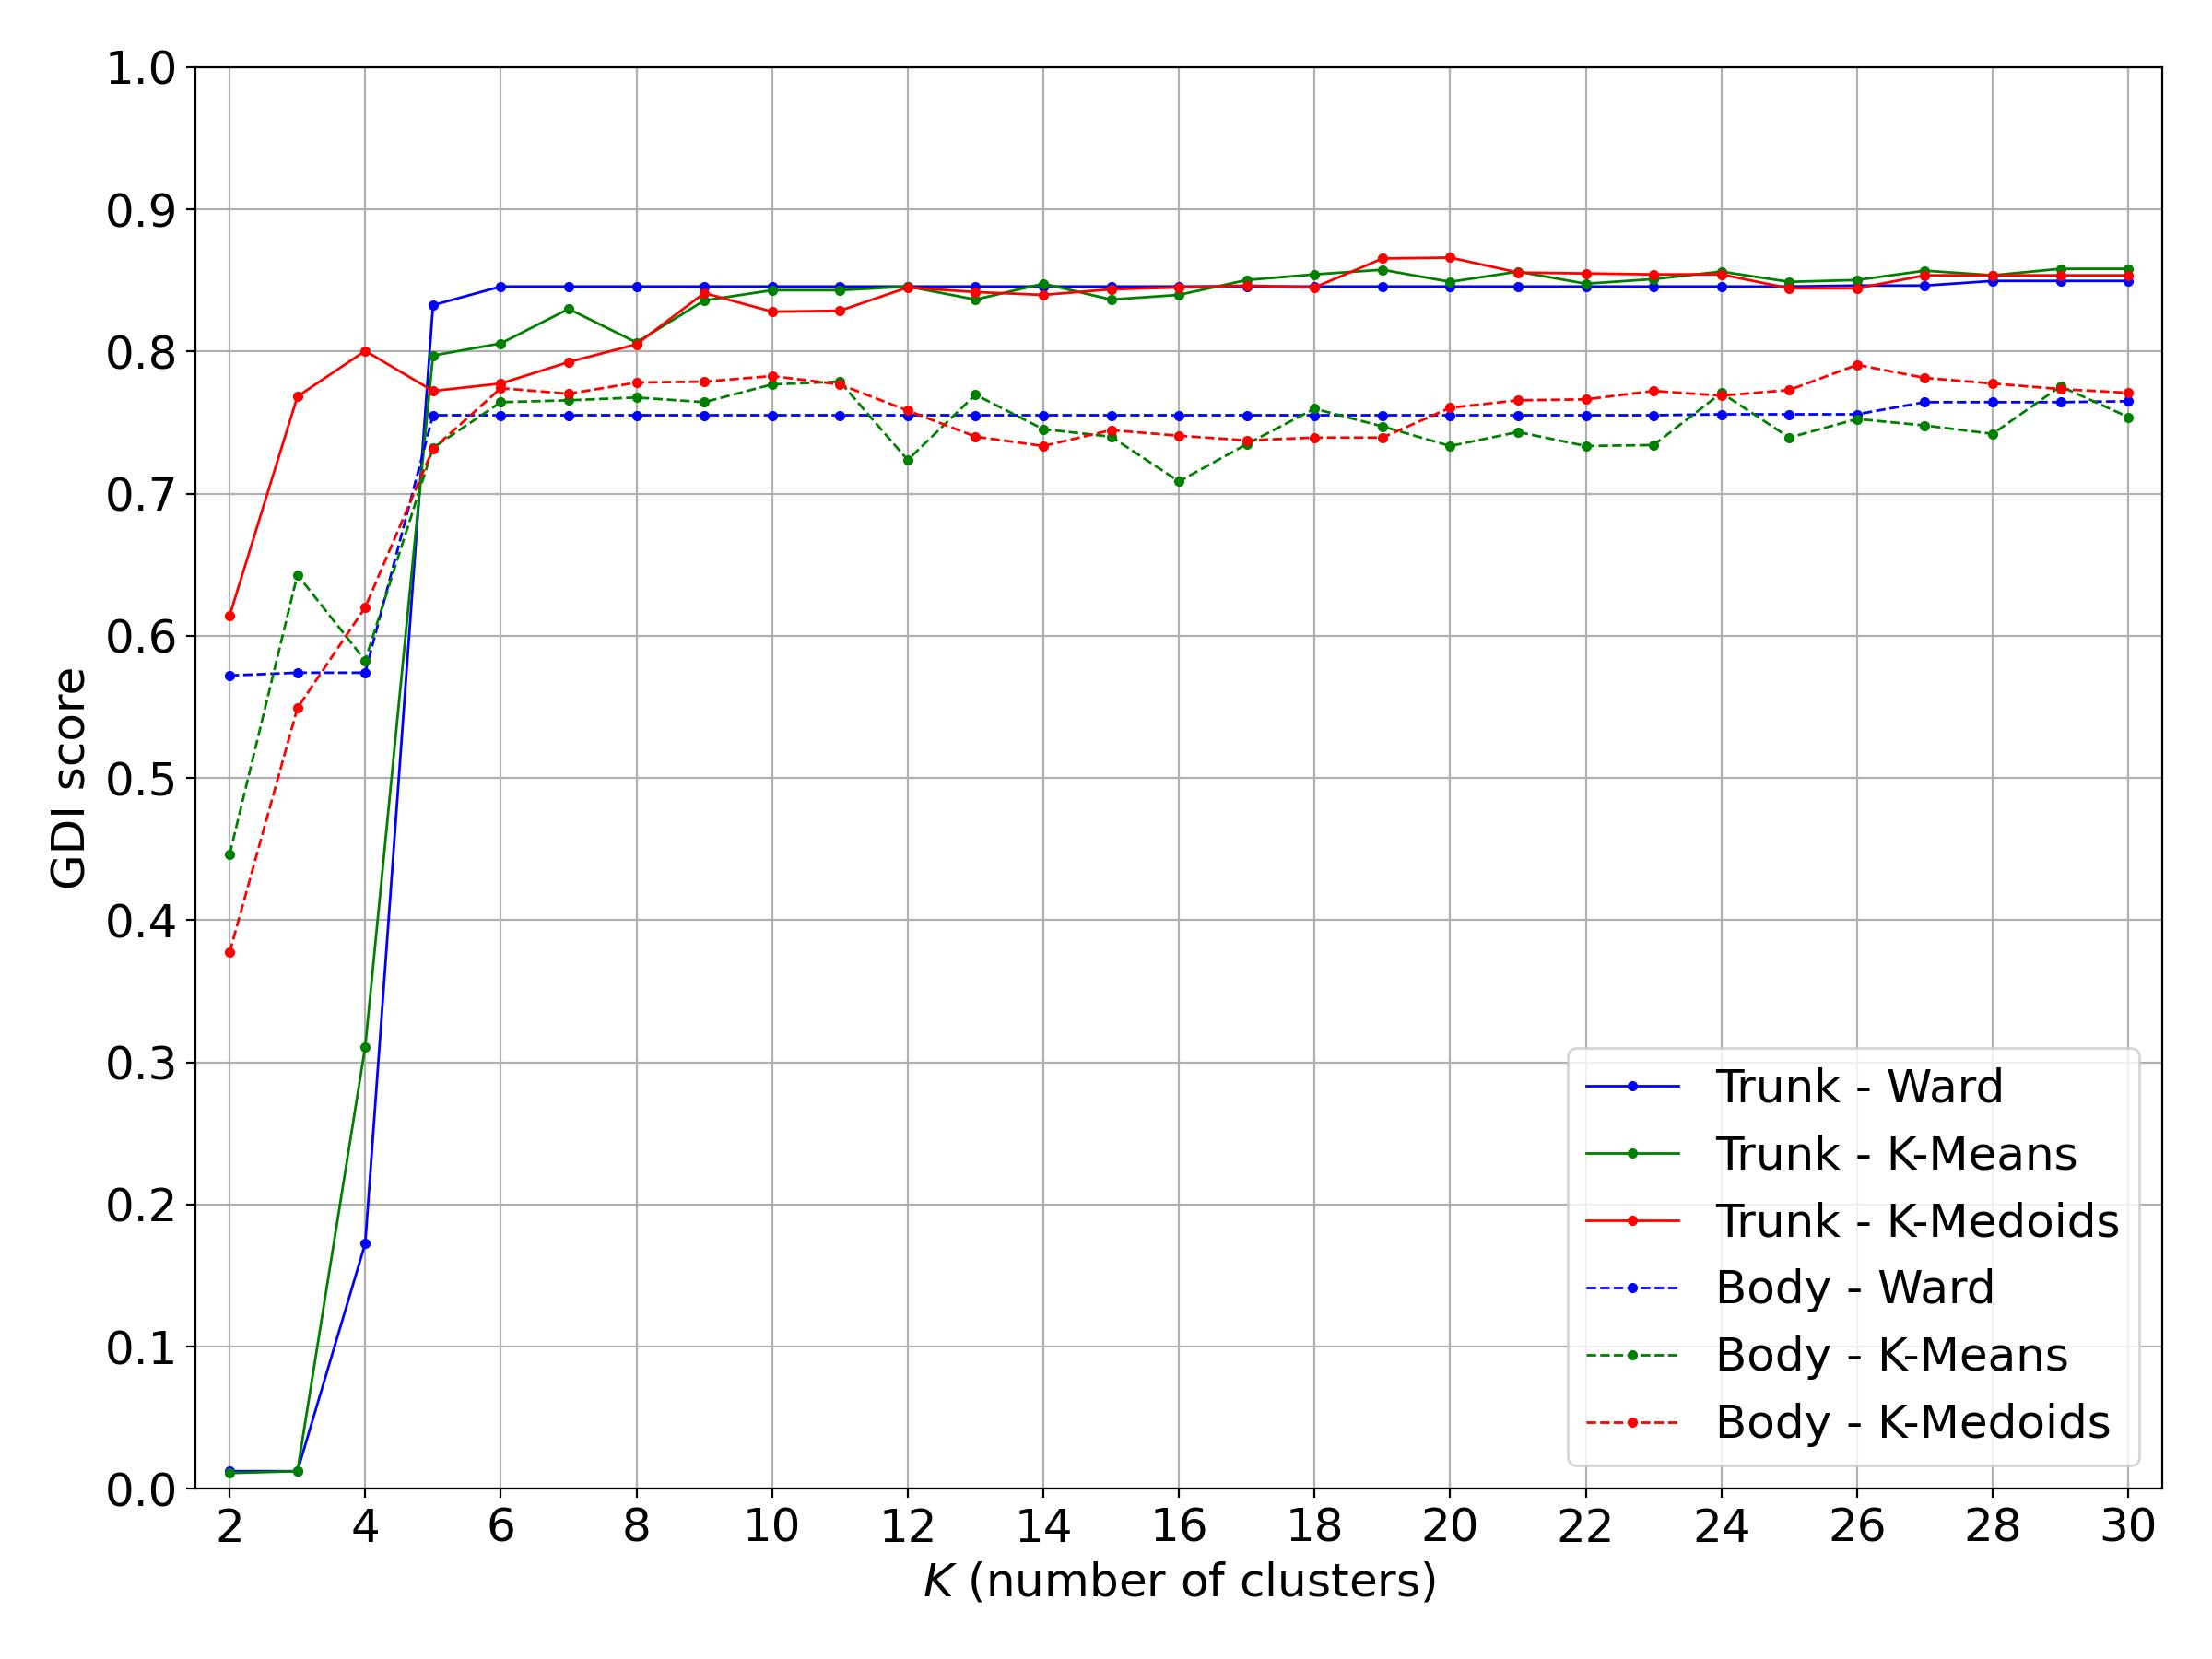
\includegraphics[width=.49\textwidth]{img/GDI/TSMFGDI}
	\caption{Comparison of GDI score on the persistence silhouettes of the whole body and the trunk.}
	\label{Fig:gdi_S_BT}
\end{figure}

From the curves of Figure \ref{Fig:gdi_S_BT} and the average GDI scores of Table \ref{Tab:gdi_S_BT}, it appears that for clustering based on silhouette persistence vectors, it is worth restricting to trunk points, particularly for K-Medoids clustering.

%\subsubsection{Conclusion}
%Based on the GDI score to choose the clustering method, the K-Medoid clustering (PAM) applied to the trunk points seems to be the best.

\section{Human body shapes classification} \label{sec:classification}

%In this section we use clustering algorithms on men and women separately in order to define types of human body shapes.

\subsection{Male morphotypes}

To define morphotypes of men body shapes, we perform a Ward-linkage hierarchical clustering on silhouettes of the persistence diagrams of the men point clouds together with the euclidean distance. The associated dendrogram is given in Figure \ref{fig:dendrogram_H}.

\begin{figure}[H]
    \centering
    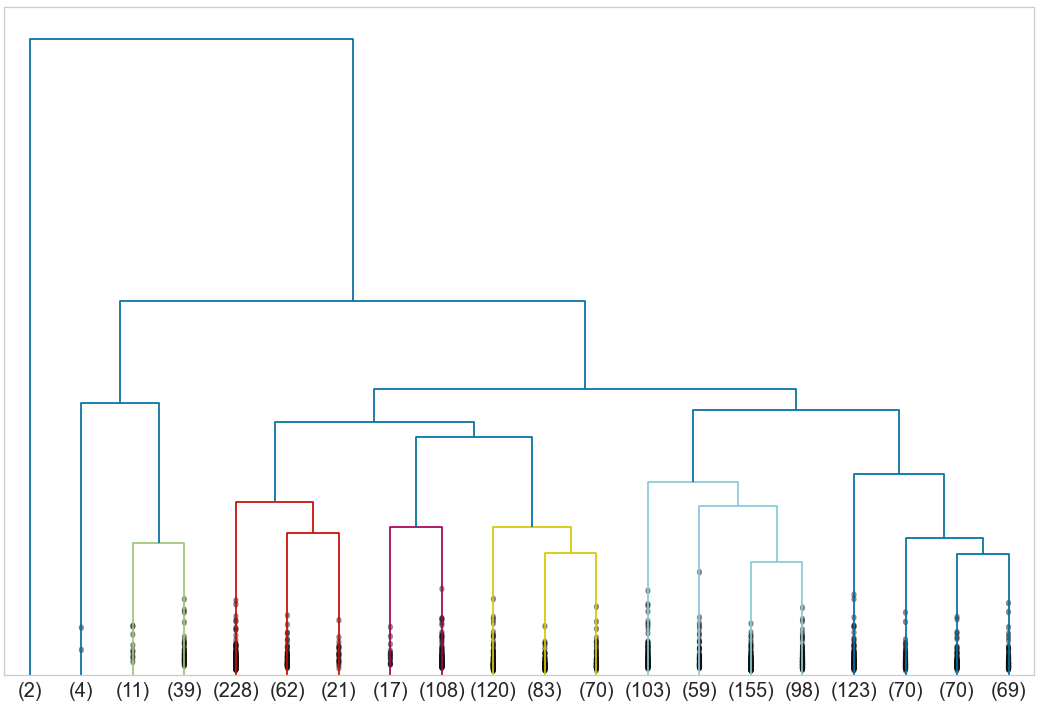
\includegraphics[width=.49\textwidth]{img/morphotypes/H_dendrogram.png}
    \caption{Dendrogram associated to a Ward-linkage hierarchical clustering of the silhouettes of the persistence diagrams of men point clouds.}
    \label{fig:dendrogram_H}
\end{figure}

To find a correct truncation of the dendrogram we use the following clustering quality indices:
\begin{itemize}
\setlength\itemsep{-0.25em}
    \item the Elbow method;
    \item the Davies-Bouldin index \cite{DB79};
    \item the Silhouette index \cite{R87};
    \item the Dunn index \cite{D73}.
\end{itemize}

Since there is a continuity between human body shapes there is no distinguished point common to all these indices. However, the Davies-Bouldin and Dunn indices suggest both to truncate at 8 clusters. Informations about size, mean distance of all pairs, diameter, mean distance to the mean and distance between the mean and the medoid of each cluster are given in Table \ref{tab:clustering_men}.

\begin{table}[H]
\centering
\begin{tabular}{|@{\hspace{1.1mm}}c@{\hspace{1.1mm}}|@{\hspace{1.1mm}}c@{\hspace{1.1mm}}|@{\hspace{1.1mm}}c@{\hspace{1.1mm}}|@{\hspace{1.1mm}}c@{\hspace{1.1mm}}|@{\hspace{1.1mm}}c@{\hspace{1.1mm}}|@{\hspace{1.1mm}}c@{\hspace{1.1mm}}|@{\hspace{1.1mm}}c@{\hspace{1.1mm}}|@{\hspace{1.1mm}}c@{\hspace{1.1mm}}|@{\hspace{1.1mm}}c@{\hspace{1.1mm}}|}
 \hline
Cluster & $C_1$ & $C_2$ & $C_3$ & $C_4$ & $C_5$ & $C_6$ & $C_7$ & $C_8$ \\ \hline
Size & 2 & 4 & 50 & 311 & 125 & 273 & 415 & 332  \\ \hline
\begin{tabular}{@{}c@{}} Proportion \\ (in percent) \end{tabular} & 0.1 & 0.3 & 3 & 21 & 8 & 18 & 27 & 22 \\  \hline
\begin{tabular}{@{}c@{}} Mean \\ distance \end{tabular} & 79.6 & 39.4 & 28.6 & 17.4 & 20.3 & 16.3 & 18.9 & 19.4 \\ \hline
Diameter & 79.6 & 53.9 & 62 & 49.6 & 59.2 & 54.6 & 67.1 & 69.4 \\ \hline
\begin{tabular}{@{}c@{}} Distance \\ to the mean \end{tabular} & 39.8 & 24.4 & 19.6 & 12.1 & 14.2 & 11.5 & 13.1 & 13.6 \\ \hline
\begin{tabular}{@{}c@{}} Distance \\ mean-medoid \end{tabular} & 39.8 & 20.1 & 9 & 3.4 & 5.9 & 6.9 & 5.1 & 6.1 \\ \hline
\end{tabular}
    \caption{Clustering of men body shapes.}
\label{tab:clustering_men}
\end{table}

The first cluster is only composed of two individuals who are extremely overweight and their meshes are shown in Figure \ref{fig:H_cluster1}. The four men of the second cluster are also extremely overweight.

The medoid is the element minimising the distance with other elements of the cluster. It can be considered as a representative and we show in Figure \ref{fig:H_medoids} the medoids associated to every cluster, except to the first cluster.

\begin{figure}[H]
    \centering
    \subfigure[\tt S0517]{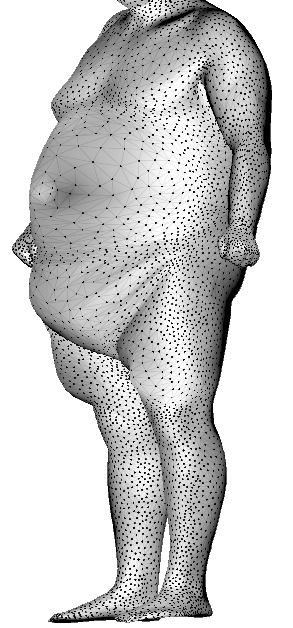
\includegraphics[height=.2\textheight]{img/morphotypes/H_medoids/H_cluster1_ind1.png}}\qquad
    \subfigure[\tt S0553]{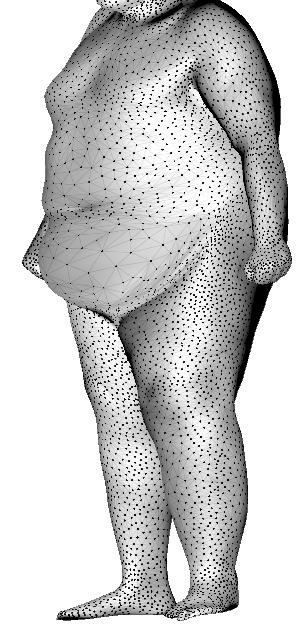
\includegraphics[height=.2\textheight]{img/morphotypes/H_medoids/H_cluster1_ind2.png}}
    \caption{The two individuals in cluster $C_1$.}
    \label{fig:H_cluster1}
\end{figure}

\renewcommand\thesubfigure{}
\begin{figure}[H]
    \centering
    %\underline{\textbf{Cluster Medoids}}\vspace{2mm}\\
    \subfigure[$(C_2)$ {\tt S2864}]{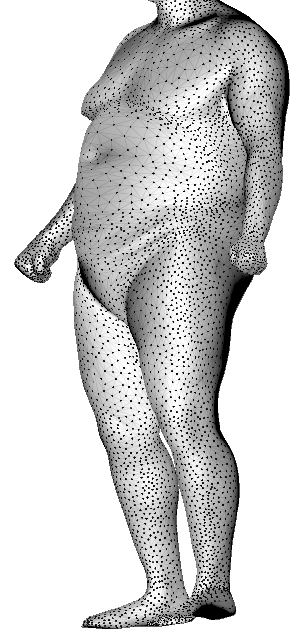
\includegraphics[height=.2\textheight]{img/morphotypes/H_medoids/H_medoid2_S2864.png}}
    \subfigure[$(C_3)$ {\tt S1502}]{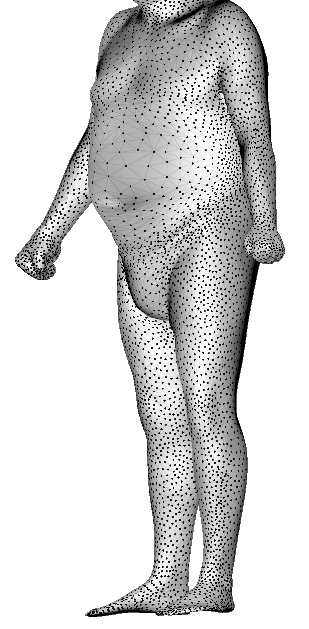
\includegraphics[height=.2\textheight]{img/morphotypes/H_medoids/H_medoid3_S1502.png}}
    \subfigure[$(C_4)$ {\tt S2055}]{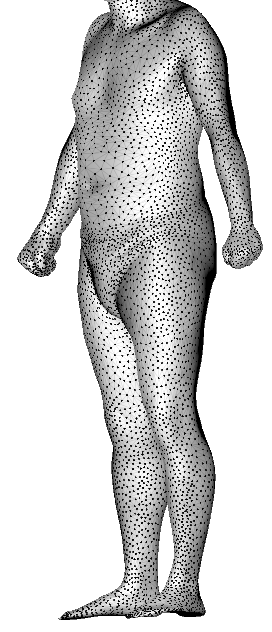
\includegraphics[height=.2\textheight]{img/morphotypes/H_medoids/H_medoid4_S2055.png}}
    \subfigure[$(C_5)$ {\tt S2640}]{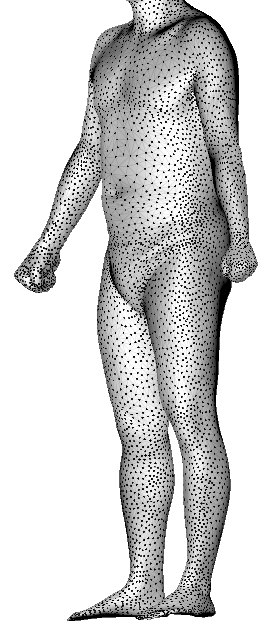
\includegraphics[height=.2\textheight]{img/morphotypes/H_medoids/H_medoid5_S2640.png}}
    \subfigure[$(C_6)$ {\tt S4286}]{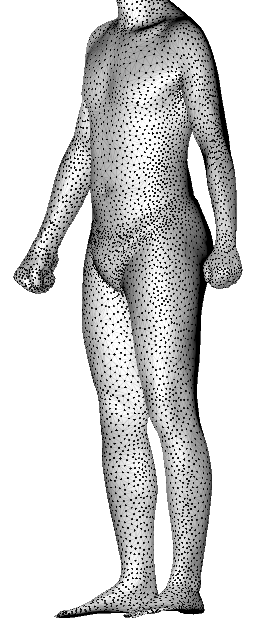
\includegraphics[height=.2\textheight]{img/morphotypes/H_medoids/H_medoid6_S4286.png}}
    \subfigure[$(C_7)$ {\tt S2982}]{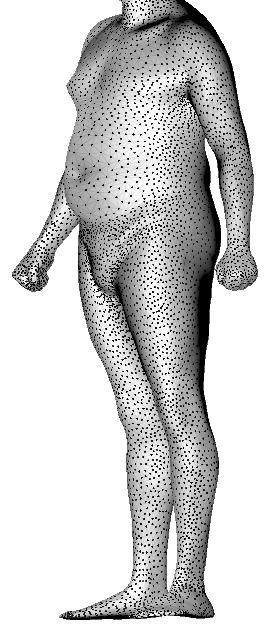
\includegraphics[height=.2\textheight]{img/morphotypes/H_medoids/H_medoid7_S2982.png}}
    \subfigure[$(C_8)$ {\tt S4505}]{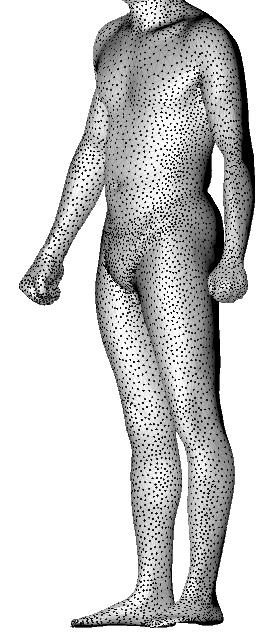
\includegraphics[height=.2\textheight]{img/morphotypes/H_medoids/H_medoid8_S4505.png}}

    \caption{Medoids of clusters $C_2$ to $C_8$ of the Ward-linkage hierarchical clustering.}
    \label{fig:H_medoids}
\end{figure}

The clusters $C_3$ and $C_7$ are composed of overweight individuals of different categories while the thinnest men are located in cluster $C_6$. It turns out that individuals of clusters $C_4$, $C_5$ and $C_8$ have a standard morphotype but that men of $C_8$ have a shorter torso than in $C_4$ and $C_8$ and that men of $C_4$ are more corpulent that in the two others.

\subsection{Female morphotypes}

Similarly, to define morphotypes of women body shapes, we perform a Ward-linkage hierarchical clustering on silhouettes of the persistence diagrams of the women point clouds together with the euclidean distance. The associated dendrogram is given in Figure \ref{fig:dendrogram_F}.

\begin{figure}[H]
    \centering
    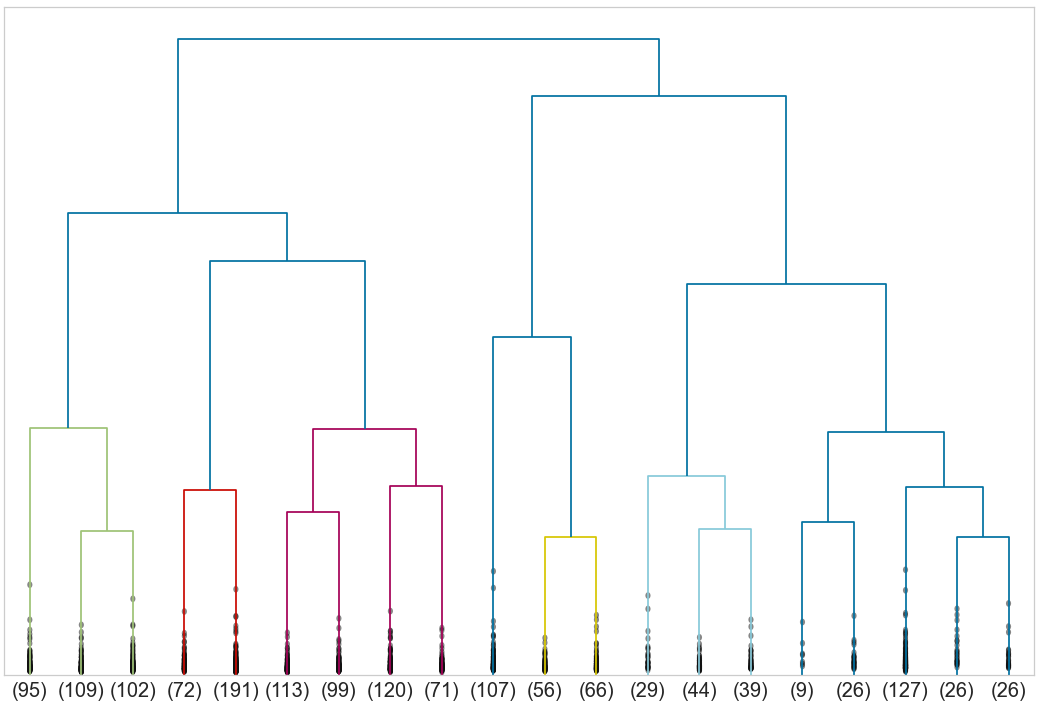
\includegraphics[width=.49\textwidth]{img/morphotypes/F_dendrogram.png}
    \caption{Dendrogram associated to a Ward-linkage hierarchical clustering of the silhouettes of the persistence diagrams of women point clouds.}
    \label{fig:dendrogram_F}
\end{figure}

This time the Silhouette and Dunn indices suggest to truncate at 7 clusters. Informations about size, mean distance of all pairs, diameter, mean distance to the mean and distance between the mean and the medoid of each cluster are given in Table \ref{tab:clustering_women}. Remark that clusters of women are more compact than clusters of men since the mean distance of pairs and diameter are much smaller.

\begin{table}[H]
\centering
\begin{tabular}{|@{\hspace{1.5mm}}c@{\hspace{1.5mm}}|@{\hspace{1.5mm}}c@{\hspace{1.5mm}}|@{\hspace{1.5mm}}c@{\hspace{1.5mm}}|@{\hspace{1.5mm}}c@{\hspace{1.5mm}}|@{\hspace{1.5mm}}c@{\hspace{1.5mm}}|@{\hspace{1.5mm}}c@{\hspace{1.5mm}}|@{\hspace{1.5mm}}c@{\hspace{1.5mm}}|@{\hspace{1.5mm}}c@{\hspace{1.5mm}}|}
 \hline
Clusters & $C_1$ & $C_2$ & $C_3$ & $C_4$ & $C_5$ & $C_6$ & $C_7$  \\ \hline
Size & 306 & 263 & 403 & 107 & 122 & 112 & 214  \\ \hline
\begin{tabular}{@{}c@{}} Proportion \\ (in percent) \end{tabular} & 20 & 17 & 27 & 7 & 8 & 7 & 14\\ \hline
\begin{tabular}{@{}c@{}} Mean \\ distance \end{tabular} & 14.2 & 12.7 & 14.1 & 14.3 & 14 & 19 & 21.3\\ \hline
Diameter & 36.6 & 32 & 32.1 & 31.9 & 38.2 & 59.3 & 62.4 \\ \hline
\begin{tabular}{@{}c@{}} Distance \\ to the mean \end{tabular} & 10.1 & 9 & 10.1 & 10.1 & 9.9 & 13.3 & 14.8 \\ \hline
\begin{tabular}{@{}c@{}} Distance \\ mean-medoid \end{tabular} & 3.4 & 3.4 & 4.5 & 3.3 & 3.6 & 5.9 & 5.2 \\ \hline
\end{tabular}
    \caption{Clustering of women body shapes.}
    \label{tab:clustering_women}
\end{table}

We show in Figure \ref{fig:F_medoids} the medoids associated to the 7 clusters.

\begin{figure}[H]
    \centering
%    \underline{\textbf{Cluster Medoids}}\vspace{2mm}\\
    \subfigure[$(C_1)$ {\tt S0522}]{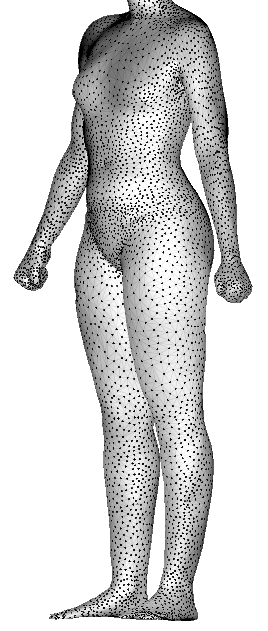
\includegraphics[height=.19\textheight]{img/morphotypes/F_medoids/F_medoid1_S0522.png}}
    \subfigure[$(C_2)$ {\tt S2018}]{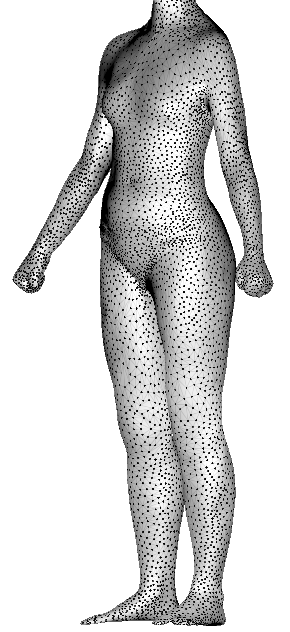
\includegraphics[height=.19\textheight]{img/morphotypes/F_medoids/F_medoid2_S2018.png}}
    \subfigure[$(C_3)$ {\tt S1604}]{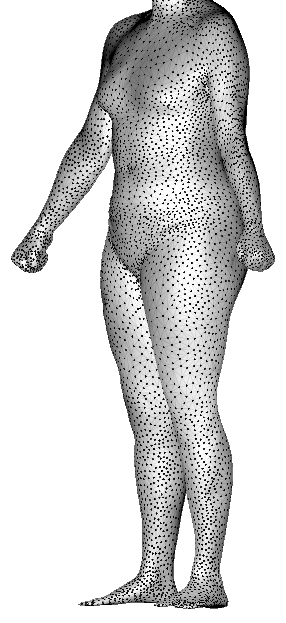
\includegraphics[height=.19\textheight]{img/morphotypes/F_medoids/F_medoid3_S1604.png}}
    \subfigure[$(C_4)$ {\tt S0174}]{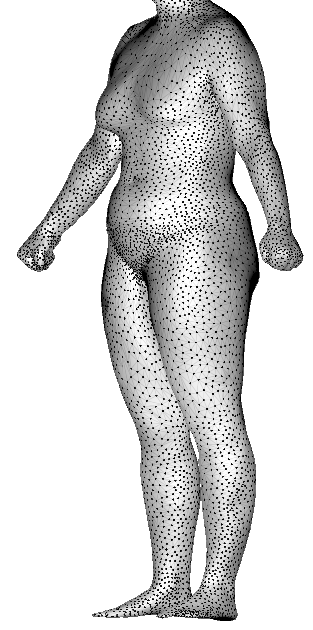
\includegraphics[height=.19\textheight]{img/morphotypes/F_medoids/F_medoid4_S0174.png}}
    \subfigure[$(C_5)$ {\tt S1076}]{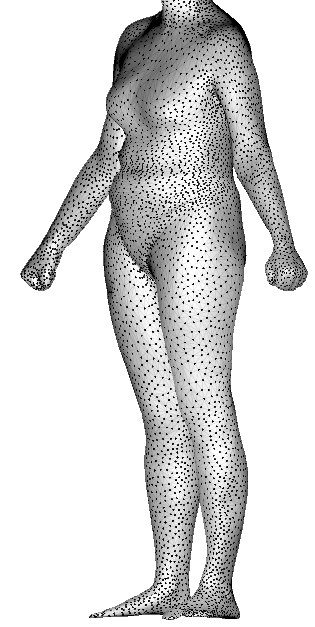
\includegraphics[height=.19\textheight]{img/morphotypes/F_medoids/F_medoid5_S1076.png}}
    \subfigure[$(C_6)$ {\tt S4507}]{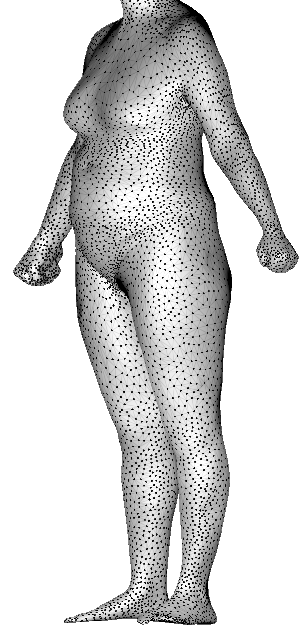
\includegraphics[height=.19\textheight]{img/morphotypes/F_medoids/F_medoid6_S4507.png}}
    \subfigure[$(C_7)$ {\tt S1174}]{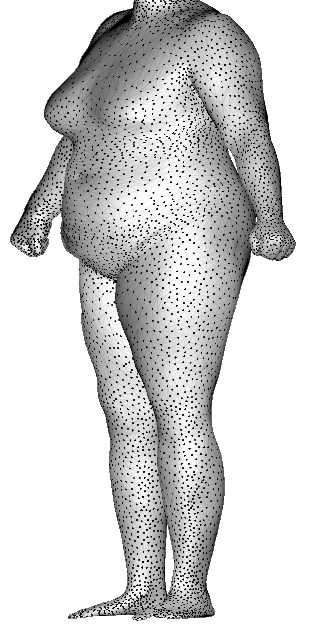
\includegraphics[height=.19\textheight]{img/morphotypes/F_medoids/F_medoid7_S1174.png}}

    \caption{Medoids of the 7 clusters of the Ward-linkage hierarchical clustering.}
    \label{fig:F_medoids}
\end{figure}

The first two clusters are composed of thin women, but in the first one they have a shorter torso with a waist circumference more pronounced. The clusters $C_6$ and $C_7$ are composed of overweight individuals of different categories. The women of the clusters $C_3$ have a straight body without much difference between waist, hip and chest circumferences. Individuals of $C_4$ and $C_5$ have an important hip circumference compared to the waist circumference but women of $C_4$ have a stronger lower body while women of $C_5$ have a shorter torso.

\section*{Acknowledgements}

This work was supported by the Joint research group in Textile Data Innovation LabCom-DiTeX.

\newpage
{\small
\bibliographystyle{ieeetr}
\bibliography{biblio}
}
\end{document}
